\documentclass{UoNMCHA}
\usepackage[authoryear]{natbib}
\usepackage{setspace}
\usepackage{array,booktabs} % For nice tables
\usepackage{amsmath,amsfonts,amssymb} % For nice maths
\newcommand{\norm}[1]{\left\lVert#1\right\rVert}
\usepackage{color}
\usepackage{enumerate}
\usepackage{listings}
\usepackage[export]{adjustbox}
\usepackage{subfig}
\usepackage{hyperref}
\usepackage[nameinlink,noabbrev]{cleveref}
\usepackage{pdfpages}
\usepackage{rotating}
\usepackage[parfill]{parskip}   % For replacing paragraph indenting with a newline instead
% Number equations per section
\numberwithin{equation}{section}
\doublespacing
\hypersetup{
%    bookmarks=true,         % show bookmarks bar?
%    unicode=false,          % non-Latin characters in AcrobatÕs bookmarks
%    pdftoolbar=true,        % show AcrobatÕs toolbar?
%    pdfmenubar=true,        % show AcrobatÕs menu?
%    pdffitwindow=false,     % window fit to page when opened
%    pdfstartview={FitH},    % fits the width of the page to the window
%    pdftitle={My title},    % title
%    pdfauthor={Author},     % author
%    pdfsubject={Subject},   % subject of the document
%    pdfcreator={Creator},   % creator of the document
%    pdfproducer={Producer}, % producer of the document
%    pdfkeywords={keyword1} {key2} {key3}, % list of keywords
%    pdfnewwindow=true,      % links in new window
    colorlinks=true,       % false: boxed links; true: colored links
    linkcolor=blue,          % color of internal links
    citecolor=blue,        % color of links to bibliography
%    filecolor=magenta,      % color of file links
    urlcolor=blue           % color of external links
}

\definecolor{MATLABKeyword}{rgb}{0,0,1}
\definecolor{MATLABComment}{rgb}{0.1328125,0.54296875,0.1328125}
\definecolor{MATLABString}{rgb}{0.625,0.125,0.9375}

\lstset{language=Matlab,
    basicstyle=\small\ttfamily,
    keywordstyle=\color{MATLABKeyword},
    %identifierstyle=,
    commentstyle=\color{MATLABComment},
    stringstyle=\color{MATLABString},
    numberstyle=\tiny,
    %numbers=left,
    basewidth=0.5em}

\firstpage{1}    % Set page number for first page
\UoNMCHAreportNo{MECH4841 Part B} %Report number
\UoNMCHAyear{2013}   % Year
\shorttitle{FYP Report - Optical Flow Based Obstacle Avoidance} %For odd pages
%%%%%%%%%%%%%%%%%%%%%%%%%%%%%%%
\begin{document}

\includepdf[pages=-]{FYP_Cover_Page.pdf}
\title{Optical Flow Based Obstacle Avoidance for a Fixed Wing UAV\\ \ \\
{\small Final Year Project Report - MECH4841 Part B  \\June 2019}}
\author[UoNMCHA]{Patrick Prell}
\address[UoNMCHA]{
Student of Mechatronics Engineering,\\
The University of Newcastle, Callaghan, NSW 2308, AUSTRALIA \\
Student Number: 3204734 \\
E-mail: \href{mailto:Patrick.Prell@uon.edu.au}{\textsf{Patrick.Prell@uon.edu.au}}}
%%%%%%%%%%%%%%%%%%%%%%%%%%%%%%%
\maketitle
\onecolumn

\vspace{-5mm}
\section*{Abstract}
\vspace{-3mm}
Remember that executive summary may include the following information:
\begin{itemize}
    \item Defines the intention of the report.
    \item Places the report in context so the reader knows why it is important to read it.
    \item Why is it important?
    \item What problem is addressed?
    \item Briefly states the results
    \item Briefly presents the implications and recommendations
\end{itemize}
\newpage
\tableofcontents
%%%%%%%%%%%%%%%%%%%%%%%%%%%%%%%
\newpage
\lstlistoflistings
%%%%%%%%%%%%%%%%%%%%%%%%%%%%%%%
\newpage
\section{Introduction}

Exploring and navagating unknown environments is an essential instinct in biology and avoiding obstacles is an major component. For robotic vehicles to perform high level tasks, they must also have these instincts.

\begin{itemize}
    \item \textbf{Position}: Show there is a problem and that it is important to solve it.
    \item \textbf{Problem}: Describe the specifics of the problem you are trying to address
    \item \textbf{Proposal}: Discuss how you are going to address this problem. Use the literature to back-up your approach to the problem, or to highlight that what you are doing has not been done before
\end{itemize}

The rest of the report is organised as follows. \Cref{sec:Background} describes items related to the core content. \Cref{sec:Conclusion} concludes the report. Appendix~ shows an example of how to make a Table.

% %%%%%%%%%%%%%%%%%%%%%%%%%%%%%%%
\newpage
\section{Background}\label{sec:Background} %Checked with grammarly
To the average human or most mammals for that matter, visual tasks such as identifying objects and interpreting visual cues might seem like a trivial task. However, implementing algorithms that mimic a mammalian visual cortex is infuriatingly difficult and largely remains an unsolved problem \citep{hartley2003multiple}. One fact often overlooked is that for all of its amazing abilities, approximately 1/3 of the human brain is dedicated to analysing information collected from our eyes. This statistic helps to put into perspective how challenging the field of computer vision can be.

The concept of computer vision has been explored since the inception of artificial intelligence in the late 1960s. Computer vision was made possible by leaps in computer power, allowing manipulation of large (for the time) data sets such as images and videos. The following decade saw research attempting to extract information from a sequence of images using visual cues embedded in the motion of an image. This brought about research on visual navigation as a viable method for a mobile robot to navigate an environment. Using Visual Navigation on a robot to move through an unstructured environment with no prior knowledge of the map is often based on optical flow. A motion field is estimated from fusing the motion of the robot with the motion of the pixels of a video feed. Furthermore, visual navigation techniques have been inspired by biology. Observing the way that animals and insects utilise their visual systems to move about and map their environments, the processes for which this is achieved can be replicated and implemented on a robotic system \citep{altshuler2018comparison}.

The following section builds the background knowledge required to utilise visual cues as input to an obstacle avoidance system. In particular, a history of visual navigation is outlined;  the geometry of a camera and the tools for calibrating it are introduced; and the kinematics of vision optical flow and optical flow on the view sphere. Finally, this section discusses the approach taken to validate the obstacle avoidance algorithm.

\newpage
\subsection{Optical Flow}
In computer vision, we are constantly running into the problem of dimensional compression. A lot of information is lost in the projection from 3-dimensions to a 2-dimensional plane, and when that projection is inverted, the lost data needs to be inferred. In the case of optical flow, the lost data comes mainly from different assumptions that are made to make the optical flow algorithm solvable. Each Optical flow algorithm has its own set of assumptions and constraints.

Beginning with a basic description of optical flow. Optical flow is the apparent movement of objects, textures and edges between a sequence of frames. Optical flow can be thought of as the time derivative of two images. It is difficult to imagine taking the derivative of an image, and it is this which makes evaluating optical flow so difficult. One major problem with calculating optical flow is the \textit{aperture problem}. This problem manifests in many optical illusions that trick the human brain as well. An example of this effect can be seen in \cref{fig:ApertureProblem}. To an unassuming camera, it is impossible to tell the direction of the striped pattern.

\begin{figure}[ht]
    \begin{center}
        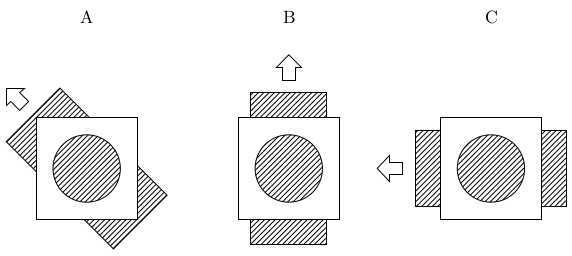
\includegraphics[width=.6\linewidth]{Figures/ApertureProblem}
        \caption{The direction of the stripes through the aperture is unclear without more context}
        \label{fig:ApertureProblem}
    \end{center}
\end{figure}

Many optical flow algorithms rely on the derivative of an image. More specifically how does the pixel intensity change from one pixel to the next: This is known as the \textit{image gradient}. Due to the intensity of an image only being defined in discrete locations, an assumption of some underlying continuous intensity function needs to be made. similar to the traditional definition of derivatives, the image gradient is separable. To calculate the partial derivatives if an image, an \textit{image kernal} is designed to capture the change intensity along each particular dimension. Optical flow requires the image gradient in $x, y$ and $t$, \cref{eq:ImageKernals} are the image kernels for these directions.

\begin{equation}\label{eq:ImageKernals}
	\frac{\delta I}{\delta x} = 
	\begin{bmatrix}
		-1 &0 &1\\
		-2 &0 &2\\
		-1 &0 &1
	\end{bmatrix},\;
	\frac{\delta I}{\delta y} = 
	\begin{bmatrix}
		-1 & -2 &-1\\
		0 & 0 & 0\\
		1 & 2 & 1
	\end{bmatrix},\;
	\frac{\delta I}{\delta t} = \underbrace{
	\begin{bmatrix}
		-1 & -1 & -1\\
		-1 & -1 & -1\\
		-1 & -1 & -1
	\end{bmatrix}}_\text{{frame $t_{0}$}} + \underbrace{
	\begin{bmatrix}
		1 & 1 & 1\\
		1 & 1 & 1\\
		1 & 1 & 1
	\end{bmatrix}}_\text{{frame $t_{1}$}}
\end{equation}

There have been many solutions proposed to calculate the motion of pixels in an image. Each method being designed for different tasks and have their own set of advantages and disadvantages in a particular situation they were designed for. Two early methods for calculating optical flow are the \textit{Horn and Schunk} optical flow algorithm and the \textit{Lucas - Kanade} method. Although both of these methods were devised over 20 years ago, they have laid a foundation for many optical flow algorithms following \citep{sun2010secrets}. The Farneback algorithm, a much more recent algorithm will then be discussed as this is the algorithm used for the project.

\subsubsection{Horn \& Schunk Optical Flow}\label{sec:HornSchunk}
Horn and Schunck optical flow is based around an assumption known as the \textit{Brightness constancy}. This says that the intencity of a pixel remains constant over a small step in time.
\begin{equation}
	\frac{dI}{dt} = 0
\end{equation}
Defining a vector field $\mathbf{h} = (u, v) = \left(\frac{du}{dt}, \frac{dv}{dt}\right)$ that hold the brightness constancy true, the chain rule is used to derive the following \textit{optical flow constraint} equation.

\begin{equation}
	\nabla I \mathbf{h} + I_{t} = 0
\end{equation}

This equation exposes the aperture problem in \ref{fig:ApertureProblem} mathematically. There are more variables to solve for than there are linearly independent equations meaning there is no unique solution for these variables. in \cite{horn1981determining}, This problem addressed by formulating the estimation of optical flow as a minimisation problem. where the vector field $(u, v)$ is presented as the minimiser for an energy function $J(u, v)$. this energy function is made up of the optical flow constraint based on brightness constancy, and another term based on the gradient of the flow. The resulting energy function is as follows:
\begin{equation}
	J(u, v) = \int_{\Omega}(I_{x}u + I_{y}v + I_{t})^{2} + \alpha^2(|\nabla u|^{2} + |\nabla v|^{2})
\end{equation}
where $\alpha$ is the weight of the smoothness of the resulting flow field.

Horn and Schunck's optical flow algorithm was a huge step forward in computer vision research, although this algorithm is limited in that it typically can only estimate small motions, the method fails in the presence of large motion when the gradient of the image is not smooth enough \citep{meinhardt2013horn}.

\subsubsection{Lucas - Kanade Optical Flow}
Since its introduction in 1981, techniques pioneered by the Lucas-Kanade method have become some of the most widely used tools for in computer vision. The main idea behind the Lucas-Kanade method is image alignment, where a region in an image is translated and deformed to minimise the least squared difference between the region and the following frame \citep{lucasKanade20yearson}. Furthermore, the Lucas-Kanade method operates under the assumption that the flow is effectively constant in a small cluster of pixels, the method can then solve the optical flow equation for all the pixels in that neighbourhood using least squares regression. The Lucas-Kanade method improved on previous methods by using the spatial intensity gradient to find the disparity vector $h$, reducing the algorithms calculation time to $O(M^2log(N))$ for the average case \citep{rojas2010lucas}. The Lucas - Kanade Optical Flow algoithm is known as a sparce optical flow algorithm, calculating the pixel flow based on feature matching.

The goal of Lucas-Kanade optical flow algorithm is to match a subset of pixels $\mathbf{T}(x)$ from an image at time $t_0$ to a subsequent template image $\mathbf{I}(x)$ at time $t_1$. The necessary movement of $\mathbf{T}(x)$ becomes the optical flow for that region. 

Considering a frame $I(x, y)$, assuming only small motion occurs between the time step, The new image can be represented as $H(x, y) = I(x + \delta x, y + \delta y)$. Finally, by using a Taylor series expansion the Lucas-Kanade equation can be written as:
\begin{equation}
	\begin{bmatrix}
		\sum{I_{x}I_{x}} & \sum{I_{x}I_{y}} \\
		\sum{I_{x}I_{y}} & \sum{I_{y}I_{y}}
	\end{bmatrix}
	\begin{bmatrix}
		\delta x \\
		\delta y
	\end{bmatrix} = -
	\begin{bmatrix}
		\sum{I_{x}I_{t}}\\
		\sum{I_{y}I_{t}}
	\end{bmatrix}
\end{equation}
where $\delta x$ and $\delta y$ is the flow in thier respective directions.

Similar to the horn and Schunk method in \cref{sec:HornSchunk}, assumptions must be made to solve this equation. the two main assumptions made to constrain the equation are, the brightness constancy, mentioned in \cref{sec:HornSchunk} and a \textit{spacial coherance} constraint. The spacial coherance encapulates the idea that there are regions within the image where all the pixels are moving relative to each other.

\subsubsection{Farneback Optical flow}
A more recent algorithm for calculationg optical flow is presented by Gunnar Farneback. This method is based on the quadratic polynomial expansion transform. The idea begind the Farneback algorithm is to model an image as a function by locally fitting a polynomial to the image at each pixel. The polynomial expansion allows a neighbourhood for each pixel to be aproximated \cite{farneback2003two}. The signal model used in the Farneback algorithm is given by:
\begin{equation}
	f(\mathbf{x}) \approx \mathbf{x}^{\top}\mathbf{A}\mathbf{x} + \mathbf{\vec{b}}^{\top} + c
\end{equation}
where $\mathbf{x}$ is the local pixel coordinates, $\mathbf{A}$ is a symetric matrix. A least squares fitting for the pixel nebourhood is then performed to find the coefficents. Due to theis polynomial being based on a window surrounding each pixel, there is a weighting applied making the function more sensitive to pixels closer to the centre of the window. For this reason the choise of the neibourhood size is an important consideration as it determins the scale of the features that this algorithm is sensitive to. \cref{fig:farnebackAlgorithm} shows the opperation of the Farneback algorithm as a one dimentional hystogram, where the height $y$ at each point represents the pixel intensity as in the 2-dimensional case and.

\begin{figure}[ht]\label{fig:farnebackAlgorithm}
    \begin{center}
        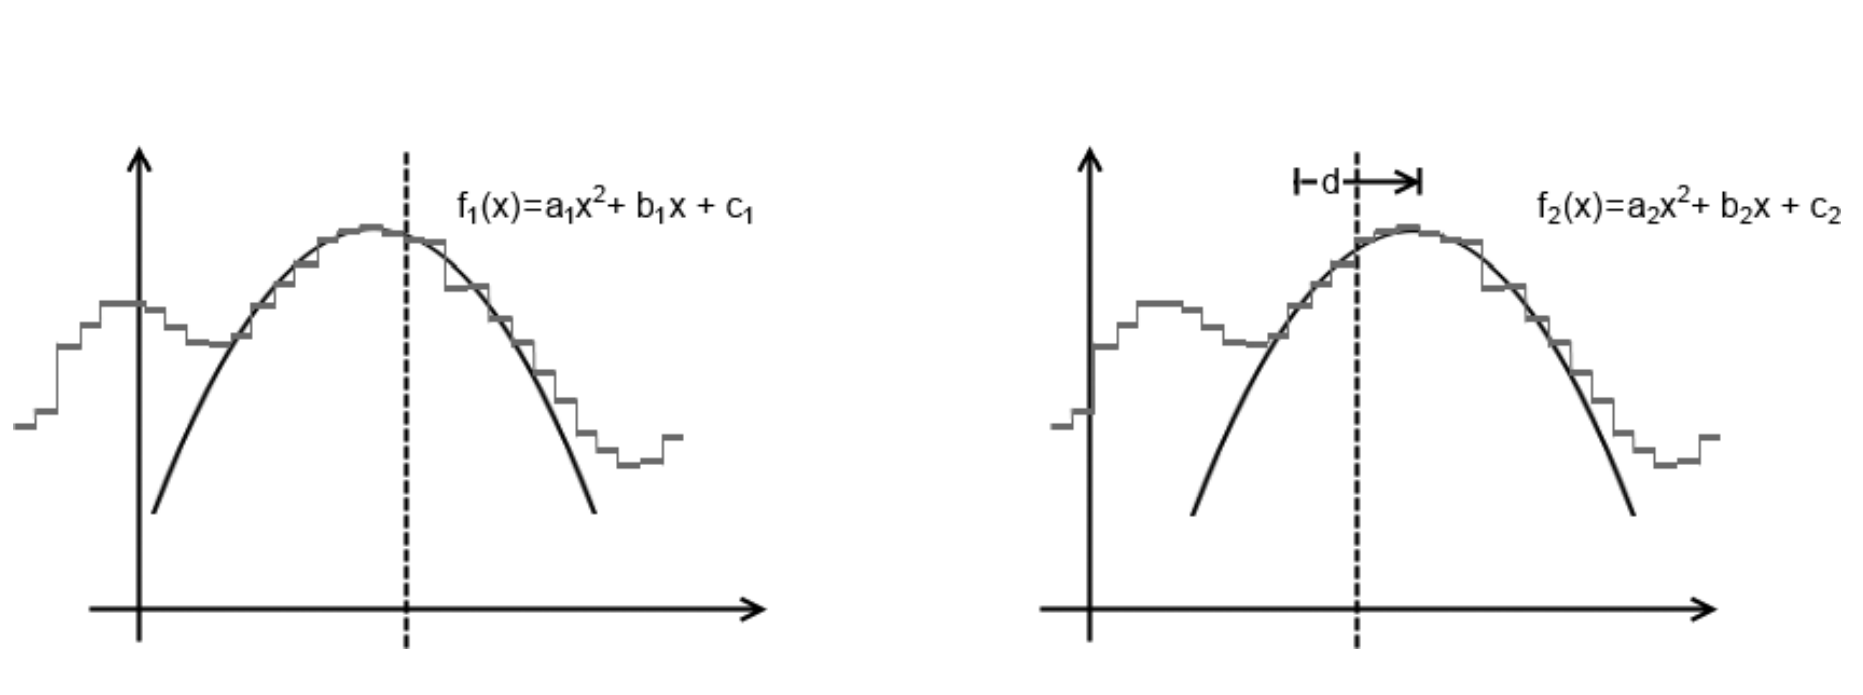
\includegraphics[width=1\linewidth]{Figures/farnebackAccuracy}
        \caption{A one dimentional illustration of the Farneback algorithm. $I_{t0}$ (left) shows the image before a displacement $d$ and $I_{t1}$ shows the image after. Image from \citep{learningOpenCV}}
    \end{center}
\end{figure}
The resulting quadratic polynomials from one timestep to the next, $f_{1}$ and $f_{2}$ in \cref{fig:farnebackAlgorithm}, can be related through the equations:
\begin{equation}
	\begin{split}
		a_{1} &= a_{2}\\
		b_{1} &= b_{2} + 2a_{1}\\
		c_{1} &= c_{2} + b_{1}d-a_{1}d^{2}
	\end{split}
\end{equation}
The displacement $d$ can then be solved for through:
\begin{equation}
	d = -\frac{1}{2a_{1}}(b_{2}-b_{1})
\end{equation}
There is a probelm with this aproach on its own, that is this method will only work for movement that can be captured in the neibourhood chosen for the polynomial. However this issue can be resolved if dome information about the displacement is already known, for instance from a previous calculation of the algorithm. So rather than comparing two images at the same point, It is possible to compare the points based on an estimated displacement, and refine the results form there. Another method for dealing with large movements is a pyramydal aproach. This involves calculating the flow on a pair of lower resolution images where large movement apears small. This aproximation can then be refined by feeding the results forward to higher order pyramids \citep{learningOpenCV}.

\begin{figure}[ht]\label{fig:farnebackYosemite}
    \begin{center}
        \includegraphics[width=.6\linewidth]{Figures/farnebackYosemite}
        \caption{Results from the Farneback Optical flow algorithm run on the Yosemite optical flow evaluation sequence\citep{farneback2003two}}
    \end{center}
\end{figure}

\begin{figure}[ht]\label{fig:farnebackResults}
    \begin{center}
        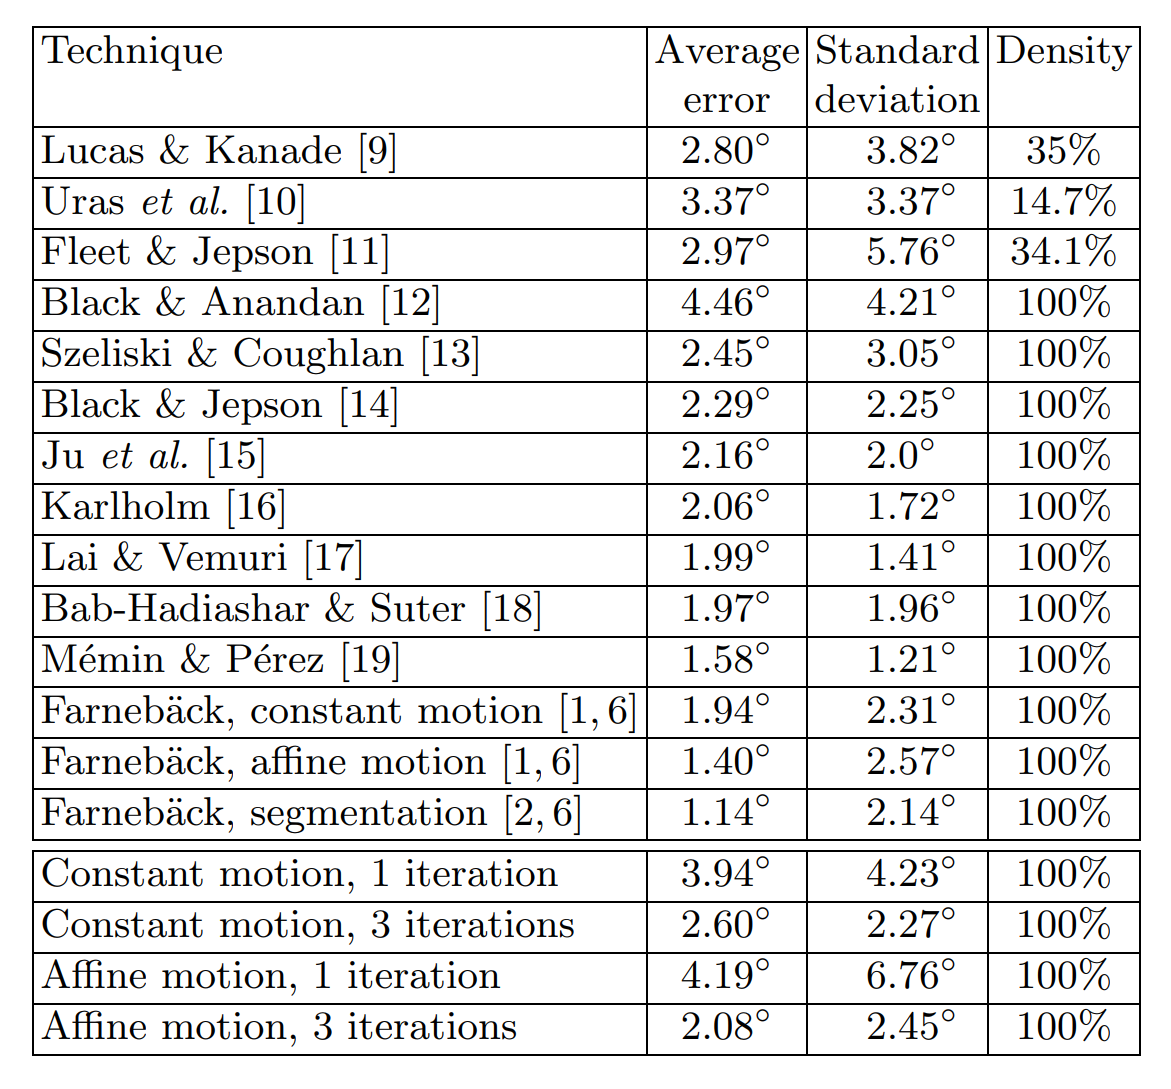
\includegraphics[width=.5\linewidth]{Figures/farnebackResults}
        \caption{Farneback Algorithm compared with Lucas-Kanade, Horn \& Schunk along with many other methods not discussed \citep{farneback2003two}}
    \end{center}
\end{figure}

The Farneback algorithm was evaluated against a common optical flow evaluation dataset known as Lynn Quam’s Yosemite sequence. This dataset is a synthetic sequence of images with a known motion field, against which an algorithm can be evaluated. Furthermore, the dataset features discontinuity at oclution boundaries and depth variation. \cref{fig:farnebackYosemite} and \cref{fig:farnebackResults} show the results obtained by \cite{farneback2003two}.
\subsubsection{What is Observable in Optical Flow}

\subsection{Visual Navigation}\label{sec:visualNavigation}
For the majority of autonomous rovers the navigation system is the key component to successfully carrying out its task. The rover collects data about its environment from sensors on the platform, attempting to extract meaningful information about its own state, such as its inclination and position relative to some reference. These sensors have typically included inertial measurment units (IMU), global positioning systems (GPS) and light detection and rainging (LiDAR) devices \citep{wang2015obstacle}.

Visual navigation refers to the technique of navigationg an environment, primarily using input from a vision sensor such as a camera \citep{chatterjee2012vision}. Navigating an environemt sucessfully relys on the rover having an understanding of the relationship between its actions and the environment surrounding it. And it is this relationship that is so dificult to design into an algorithm \citep{zhu2017target}. In recent years, the use of cameras on autonomous vehicle has drastically increased thanks to the increased availability of camera hardware to the average hobbiest. The advent of more accessable hardware means that much more attention has been places on the task of designing an algorithm to interprate the data form a robotic vision system.

\subsubsection{Inverse Optimal Control}\label{sec:IOC}
The traditional way of designing an autonomous system is to create a cost function for the system and use this cost function to produce an optimal policy. This method often involves tweaking tuning prametrs and weight values that are too complicated to understnd intuitively \citep{ratliffinverse}. This is known as optimal control. as the name suggests, inverse optimal control flips these techniques around. Inverse optimal control can be a far more intuitive method of obtaining the desired behavior from a robot.

Rather than defining a cost function that generates the policy for the robot, inverse optimal control uncovers the cost function that best explains demonstrated optimal behavior \citep{ratliffinverse}. This behavior is derived from from expert demonstrations of the optimal policy \citep{levine2012continuous}. In nature, there are many systems found that have all ready implemented a near optimal control stratergy for many visual tasks. The question that inverse optimal control answers is, how can we attempt to mimic the behavior seen nature for the purposes of our goals.

To begin 

\subsubsection{Biomimicry}
Biology so often holds a wealth of inspiration for engineers. From the material science of the microstructures in a butterfly wing to the computational fluid dynamics of a Kingfisher diving into water \citep{benyus1997biomimicry}. visual sensors are found so frequently in nature, making it very productive to look at nature and tap into the eons of knowledge distilled by evolution.

Due to the immense complexity of understanding and implementing a vission based navigation system, reaserchers have looked to honeybees for clues. Honeybees have been noticed to display superb agylity and remarkable compitency in navigationg their environment \citep{srinivasan2012biology}. Using an inverse optimal control framework, the interpritation that the honeybee has of its environment was investigated. Reaserchers at the university of queensland were able to devise and setup an experiment (\cref{fig:BeeExperiment}) with the goal of deducing how a bee negotialtes its environment.

\begin{figure}[ht]
    \begin{center}
        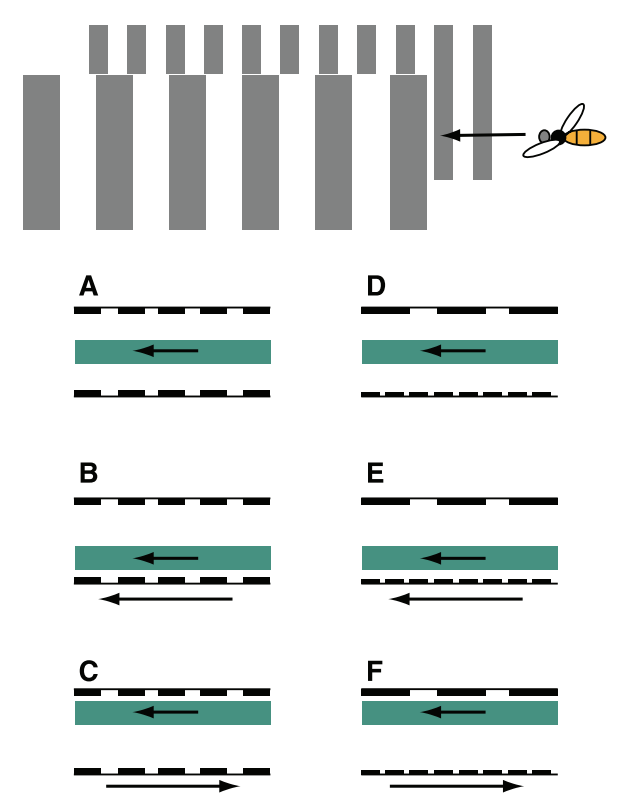
\includegraphics[width=.6\linewidth]{Figures/beeExperiment}
        \caption{Inverse optimal control experiment used to identify the mechanism that bees use to maintain their distance to a wall}
        \label{fig:BeeExperiment}
    \end{center}
\end{figure}

\subsubsection{Trajectory Planning}

\subsection{Reference Frames and Coordinate Systems}\label{sec:ReferenceFrames}
In general, the motion of an object needs to be described relative to some coordinate system and the reference frame. Defined by \cite{3900Notes}, a reference frame is a perspective from which the motion is described by an observer. A reference frame can be defined by a set of at least 3 non-colinear points that are rigidly connected. The reference frames used in this project are $\mathcal{C}$, $\mathcal{B}$ and $\mathcal{N}$ for the camera, the vehicle (body) and the world frames respectively.

Furthermore, a coordinate system is a way to describe the position and motion of objects relative to its reference frame. A coordinate system in three-dimensional Euclidean geometry is made up of at least three orthogonal basis vectors of unit length. This report uses the same notation as used in \cite{3900Notes} to describe a vector from point $O$ to point $P$ as $\vec{r}_{P/O}$. \Cref{fig:ReferenceFrame} shows an example reference frame $\mathcal{C}$ attached to a camera with an associated coordinate system $\{c\}$.

\begin{figure}[ht]
    \begin{center}
        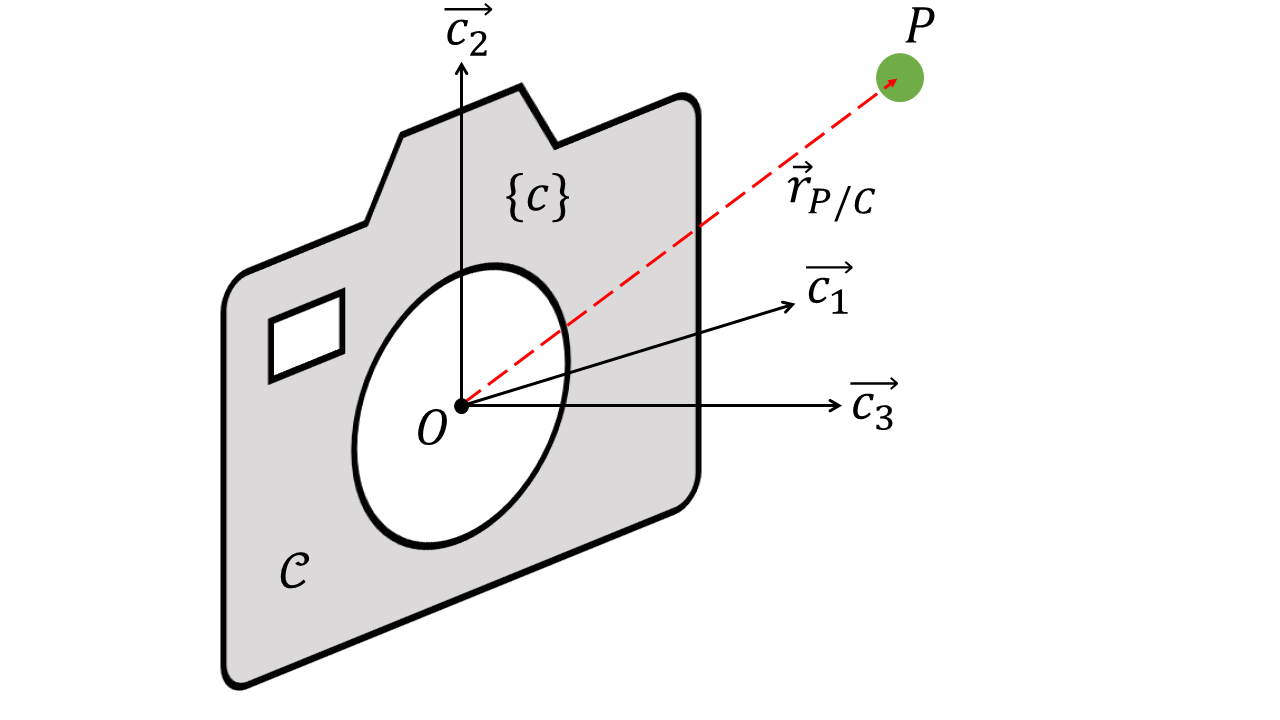
\includegraphics[width=.6\linewidth]{Figures/ReferenceFrame}
        \caption{A reference frame $\mathcal{C}$ with its associated coordinate system $\{c\}$}
        \label{fig:ReferenceFrame}
    \end{center}
\end{figure}

When designing computational models, it is often convenient to represent vectors as column matrices in $\mathbb{R}^3$. The basis of the original vector is denoted as a superscript of the matrix. That is, a vector $\vec{v}$ in basis $\{a\}$ is written as $\mathbf{v}^a$, or more generally: 
\begin{equation}
	\mathbf{v}^a = 
	\begin{bmatrix}
		v^{a}_1\\
		v^{a}_2\\
		v^{a}_3
	\end{bmatrix}
\end{equation}

In this form, the dot product of two vectors $\vec{u} \cdot \vec{v}$ (inner product) in the same basis becomes a matrix operation:
\begin{equation}
	(\mathbf{u}^{a})^{T}\mathbf{v}^{a} = 
	\begin{bmatrix}
		u^{a}_1 & u^{a}_2 & u^{a}_3
	\end{bmatrix}
	\begin{bmatrix}
		v^{a}_1\\
		v^{a}_2\\
		v^{a}_3
	\end{bmatrix}
\end{equation}

Additionally, the cross product of two vectors $\vec{w} = \vec{u}\times\vec{v}$ can be represented as the \textit{skew-symmetric} matrix of $\mathbf{u}^{a}$ multiplied by $\mathbf{v}^{a}$. That is:
\begin{equation}
	\mathbf{w}^{a} = \mathbf{S}(\mathbf{u}^a)\mathbf{v}^a
\end{equation}
The skew-symmetric operator $\mathbf{S(u)}$ arranges the elements in $u$ such that the resulting matrix is skew-symmetric.

\begin{equation}\label{eq:SkewSymmetric}
	\mathbf{S}(\mathbf{u}) = 
	\begin{bmatrix}
		0 & -u_{3} & u_{2}\\
		u_{3} & 0 & -u_{1}\\
		-u_{2} & u_{1} & 0
	\end{bmatrix}
\end{equation}

\subsubsection{Coordinate Transforms and Rotation Matrices}
This project uses multiple coordinate systems to deal with the complex geometry of the camera and vehicle. Therefore, in order to have context for measurements and actions of different sensors and actuators, their orientation needs to be transformed into the relevant coordinate system. The following report will use rotation matrices, as derived from a coordinate transform.

A vector can be described from multiple bases, for instance, $\vec{r}$ can be represented in both basis $\{n\}$ and basis $\{c\}$ as:
\begin{equation}\label{eq:uInAandB}
	\begin{split}
		\vec{r} &= r^{n}_{1}\vec{n}_{1} + r^{n}_{2}\vec{n}_{2} + r^{n}_{3}\vec{n}_{3}\\
		\vec{r} &= r^{c}_{1}\vec{c}_{1} + r^{c}_{2}\vec{c}_{2} + r^{c}_{3}\vec{c}_{3}
	\end{split}
\end{equation}

Expressing $\vec{r}$ as an inner product of the basis $\{c\}$ and $r^{n}$:
\begin{equation}
	\vec{r} = 
	\begin{bmatrix}
		\vec{c}_{1} & \vec{c}_{2} & \vec{c}_{3}
	\end{bmatrix}
	\begin{bmatrix}
		r^{c}_{1}\\
		r^{c}_{2}\\
		r^{c}_{3}
	\end{bmatrix}
\end{equation}
Finally, express both sides in $\{n\}$:
\begin{equation}
	\mathbf{r}^{n} =
	\begin{bmatrix}
        \mathbf{b}^{c}_{1} & \mathbf{b}^{c}_{2} & \mathbf{b}^{c}_{3}
	\end{bmatrix}
	\mathbf{u}^{c}
\end{equation}
This can be denoted more generally in matrix form:
\begin{equation}
	\mathbf{r}^{c} = \mathbf{R}^{c}_{n}\mathbf{r}^{n}.
\end{equation}

In robotics, it is often desirable to rotate a vector to a particular angle. The method used in this project is known as \textit{euler rotation}. Euler angles discretise a complex three-dimensional rotation into three separate planar rotations about each basis vector. The rotation matrices about each basis vector are given by:
\begin{equation}\label{eq:planarRotations}
	\begin{split}
		\mathbf{R}_{x}(\phi) &= 
		\begin{bmatrix}
			1 & 0 & 0\\
			0 & cos(\phi) & -sin(\phi) \\
			0 & sin(\phi) & cos(\phi)
		\end{bmatrix}\\
		\mathbf{R}_{y}(\theta) &= 
		\begin{bmatrix}
			cos(\theta) & 0 & sin(\theta)\\
			0 & 1 & 0 \\
			-sin(\theta) & 0 & cos(\theta)
		\end{bmatrix}\\
		\mathbf{R}_{z}(\psi) &= 
		\begin{bmatrix}
			cos(\psi) & -sin(\psi) & 0\\
			sin(\psi) & cos(\psi) & 0 \\
			0 & 0 & 1
		\end{bmatrix}
	\end{split}
\end{equation}

The order of these rotations effects the final position, for this reason in this project the common robotics convention of \textit{Roll, Pitch, Yaw} (RPY) will be used. The notation for a rotation matrix from $\{n\}$ to $\{c\}$ is given by $\mathbf{\Theta}^{n}_{c}  \triangleq \begin{bmatrix}\phi & \theta & \psi\end{bmatrix}^\top$. using the consecutive planar rotations from \cref{eq:planarRotations} we get $r^{b}_{a} = \mathbf{R}_{z}(\psi)\mathbf{R}_{y}(\theta)\mathbf{R}_{x}(\phi)r^{a}_{b} = \mathbf{R}(\mathbf{\Theta}^{n}_{c})r^{a}_{b}$. From this, the structure of a full rotation matrix:
\begin{equation}
	\mathbf{R}(\mathbf{\Theta}^{n}_{c}) = 
	\begin{bmatrix}
		c_{\psi} c_{\theta} & −s_{\psi} c_{\phi} + c_{\psi} s_{\theta} s_{\phi} & s_{\psi} s_{\phi} + c_{\psi} c_{\phi} s_{\theta}\\
		s_{\psi} c_{\theta} & c_{\psi} c_{\phi} + s_{\phi} s_{\theta} s_{\psi} &  −c_{\psi} s_{\phi} + s_{\psi} c_{\phi} s_{\theta}\\
		−s_{\theta} & c_{\theta} s_{\phi} & c_{\theta} c_{\phi}		
	\end{bmatrix}
\end{equation}
where $s  \triangleq sin(\mathbf{\cdot})$ and $c  \triangleq cos(\mathbf{\cdot})$.

Due to the orthogonality of rotation matrices, they have the property that the inverse of the rotation matrix is equal to its transpose:
\begin{equation}
	\mathbf{R}^{-1} = \mathbf{R}
\end{equation}
This is useful, as rotating a vector back to its original orientation is as simple as applying the transposed rotation matrix. That is $\mathbf{R}^{b}_{a} = \mathbf{R}^{a\top}_{b}$.

\subsubsection{Time Derivative of Vectors and Transport Theorem}\label{sec:VectorDerivitives}
The subtle difference between the time-derivative of a scalar magnitude and a vector magnitude is that the vector derivative depends on the reference frame from which they are being observed \cite{3900Notes}. \Cref{fig:vectorDerivitive} shows a vector $\vec{r}$ observed from two separate reference frames, $\mathcal{A}$ and $\mathcal{B}$.

\begin{figure}[ht]
    \begin{center}
        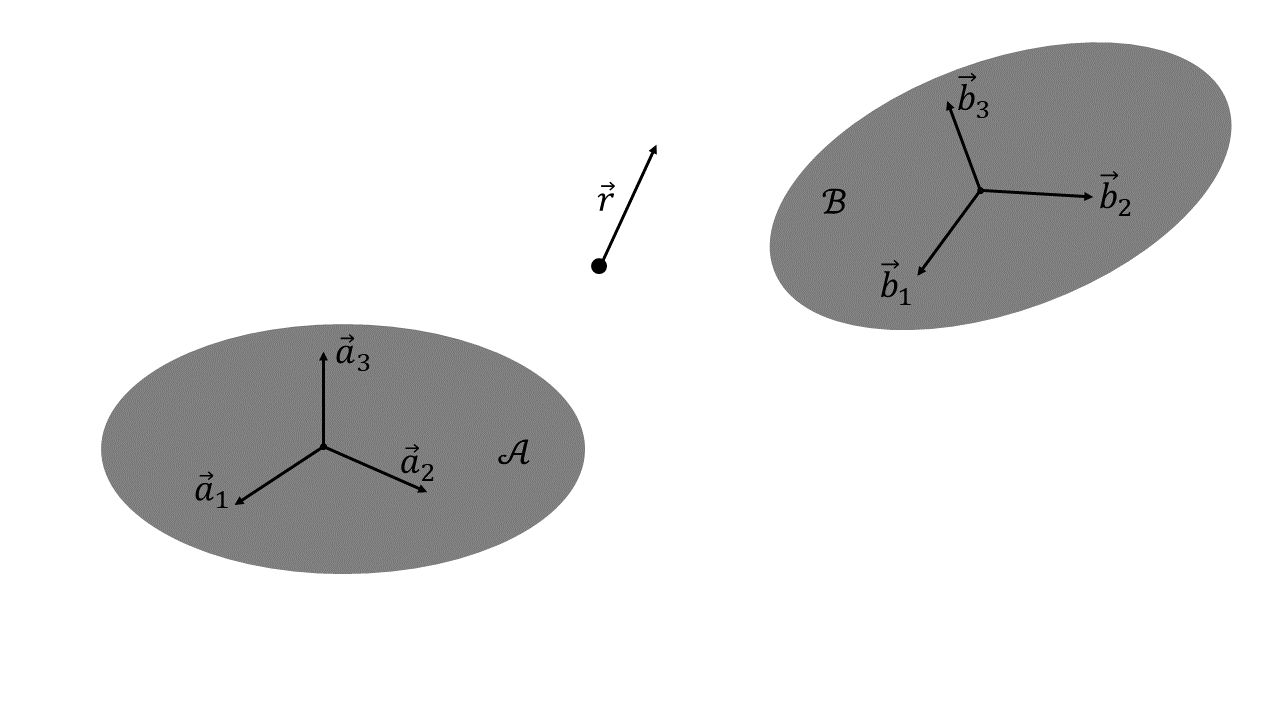
\includegraphics[width=.8\linewidth]{Figures/vectorDerivitive}
        \caption{A vector $\vec{r}$ seen from two reference frames.}
        \label{fig:vectorDerivitive}
    \end{center}
\end{figure}

Taking the time derivative of $\vec{r}$ in each vector frame:

\begin{equation}
	\begin{split}
		\frac{{}^\mathcal{A}d\vec{r}}{dt} &= \frac{dr^{a}_{1}}{dt}\vec{a}_{1} + \frac{dr^{a}_{2}}{dt}\vec{a}_{2} + \frac{dr^{a}_{3}}{dt}\vec{a}_{3}\\
		\frac{{}^\mathcal{B}d\vec{r}}{dt} &= \frac{dr^{b}_{1}}{dt}\vec{b}_{1} + \frac{dr^{b}_{2}}{dt}\vec{b}_{2} + \frac{dr^{b}_{3}}{dt}\vec{b}_{3}\\
	\end{split}
\end{equation}
Consider the case of a frisbee flying through the air carrying a spider $S$ as a passenger. Reference frame $\mathcal{F}$ is attached rigidly to the frisbee and an observer $O$ is watching it from the field in reference frame $\mathcal{O}$. Clearly, the movement of the spider is different from $\mathcal{A}$ as it is from $\mathcal{F}$ or more generally:
\begin{equation}
		\frac{{}^\mathcal{O}d\vec{r}}{dt} \neq \frac{{}^\mathcal{F}d\vec{r}}{dt}
\end{equation}
To find the time derivative of the spider relative to $\mathcal{O}$, two methods could be used: the time derivative of the vector $\vec{r}_{S/O}$ can be taken, which will prove to be a tedious exercise. Or the \textit{transport theorem} can be used.

In accordance with \cite{3900Notes}, the transport theorem states that there exists a unique vector $\vec{\omega}_{\mathcal{B}/\mathcal{A}}$ called the \textbf{angular velocity} of $\mathbf{\mathcal{B}}$ with respect to $\mathbf{\mathcal{A}}$ such that:
\begin{equation}\label{eq:transportTheorem}
	\frac{{}^\mathcal{A}d\vec{r}}{dt} = \frac{{}^\mathcal{B}d\vec{r}}{dt} + \vec{\omega}_{\mathcal{B}/\mathcal{A}}\times\vec{r}
\end{equation}
Using the transport theorem, the velocity of the spider relative to $\mathcal{O}$ is simply the velocity of the frisbee's centre $P$ plus the rotational velocity of the frisbee, resulting in:
\begin{equation}
	\frac{{}^\mathcal{O}d}{dt}\vec{r}_{S/O} = \frac{{}^\mathcal{F}d}{dt}\vec{r}_{P/O} + \vec{\omega}_{\mathcal{F}/\mathcal{O}}\times\vec{r}_{P/O}
\end{equation}

\subsection{Kinematics of Vision}
While discussing the motion of objects in a space, it is helpful to properly define a geometric definition for these points and the relative motion between them. Kinematics defines these such relationships. More specifically, kinematics defines the reference frame from which the motion of a point can be described and the transformation that associates this motion in a separate reference frame. These concepts will be used to describe the relative motion between a camera mounted on a vehicle in an environment.

\subsection{Optical Flow on the View Sphere}\label{sec:SphericalFlow}
As discussed in previous sections, optical flow used on a robotics platform is often used for navagational purposes
\begin{figure}[ht]
    \begin{center}
        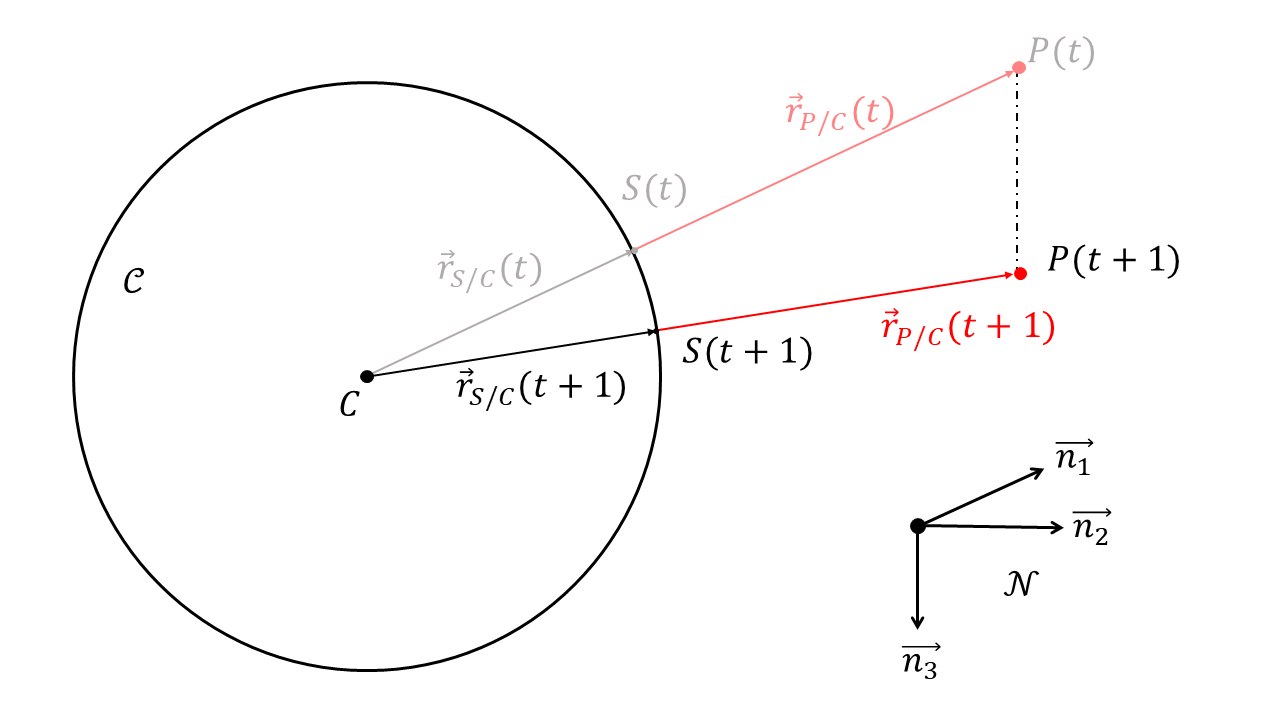
\includegraphics[width=.8\linewidth]{Figures/MeasurementModel}
        \caption{Write something here}
        \label{fig:MeasurementModel}
    \end{center}
\end{figure}
Assuming the viewsphere has a unit radius, the point $P$ can be projected onto the view sphere to point $S$ by:
\begin{equation}\label{eq:pointOnSphere}
	\vec{r}_{S/C} = \frac{\vec{r}_{P/C}}{\norm{\vec{r}_{P/C}}}
\end{equation}
Applying the concepts from \ref{sec:VectorDerivitives}, the time derivitive of $\vec{r}_{S/C}$ with respect to reference frame $\mathcal{N}$ can be taken: 
\begin{equation}
	\frac{{}^\mathcal{N}d\vec{r}_{S/C}}{dt} = \frac{{}^\mathcal{N}d}{dt}\left(\frac{\vec{r}_{P/C}}{\norm{\vec{r}_{P/C}}}\right)
\end{equation}
Noticing $\norm{\vec{r}_{P/C}}$ can be written as $(\vec{r}_{P/C} \cdot \vec{r}_{P/C})^{-\frac{1}{2}}$ and substituting this in:
\begin{equation}
	\frac{{}^\mathcal{N}d\vec{r}_{S/C}}{dt}	= \frac{{}^\mathcal{N}d}{dt}\vec{r}_{P/C}(\vec{r}_{P/C} \cdot \vec{r}_{P/C})^{-\frac{1}{2}}
\end{equation}
Now that the equation is in the form of $f(x)g(y)$ the product rule can be aplied and vector derivitives written as velocities to simplify, giving:
\begin{equation}
	\begin{split}
		\frac{{}^\mathcal{N}d\vec{r}_{S/C}}{dt} &=\frac{{}^\mathcal{N}d}{dt}\left(\vec{r}_{P/C}\right)(\vec{r}_{P/C} \cdot \vec{r}_{P/C})^{-\frac{1}{2}} + \vec{r}_{P/C}\frac{{}^\mathcal{N}d}{dt}(\vec{r}_{P/C} \cdot \vec{r}_{P/C})^{-\frac{1}{2}}\\
		\vec{v}_{S/C} &=\frac{\vec{v}_{P/C}}{\norm{\vec{r}_{P/C}}} + \vec{r}_{P/C}\frac{{}^\mathcal{N}d}{dt}(\vec{r}_{P/C} \cdot \vec{r}_{P/C})^{-\frac{1}{2}}
	\end{split}
\end{equation}

Following this, the chain rule can be applied to the second term of the equation:

\begin{equation}
	\begin{split}
		\vec{v}_{S/C} &=\frac{\vec{v}_{P/C}}{\norm{\vec{r}_{P/C}}} - \frac{1}{2} \vec{r}_{P/C}(\vec{r}_{P/C}\cdot\vec{r}_{P/C})^{-\frac{3}{2}}\frac{{}^\mathcal{N}d}{dt}(\vec{r}_{P/C} \cdot \vec{r}_{P/C})\\
		&=\frac{\vec{v}_{P/C}}{\norm{\vec{r}_{P/C}}} - \frac{1}{2} \vec{r}_{P/C}(\vec{r}_{P/C}\cdot\vec{r}_{P/C})^{-\frac{3}{2}}\left(2\vec{r}_{P/C}\frac{{}^\mathcal{N}\vec{r}_{P/C}}{dt}\right)\\
	\end{split}
\end{equation}
Again, the vector norm can be substituted back into the equation and terms collected
\begin{equation}
	\vec{v}_{S/C} =\frac{\vec{v}_{P/C}}{\norm{\vec{r}_{P/C}}} - \frac{\vec{r}_{P/C}(\vec{r}_{P/C}\vec{v}_{P/C})}{\norm{\vec{r}_{P/C}}^{3}}
\end{equation}
Rearranging \cref{eq:pointOnSphere} to get $\vec{r}_{P/C} = \vec{r}_{S/C} \norm{\vec{r}_{P/C}}$ this equation can be substituted in, and like terms canceled:
\begin{equation}
	\begin{split}
		&=\frac{\vec{v}_{P/C}}{\norm{\vec{r}_{P/C}}} - \frac{\vec{r}_{S/C}\norm{\vec{r}_{P/C}}(\vec{r}_{S/C}\norm{\vec{r}_{P/C}}\vec{v}_{P/C})}{\norm{\vec{r}_{P/C}}^{3}}\\
		\vec{r}_{S/C}&=\frac{\vec{v}_{P/C}}{\norm{\vec{r}_{P/C}}} - \frac{\vec{r}_{S/C}(\vec{r}_{S/C}\vec{v}_{P/C})}{\norm{\vec{r}_{P/C}}}
	\end{split}
\end{equation}

As previously mentioned these calculations were with respect to the world reference frame $\mathcal{N}$. However, spherical flow is measured in the camera reference frame $\mathcal{C}$. Therefore we need to apply the transport theorem outlined in \cref{eq:transportTheorem} obtaining the velocity of a point $S$ as seen from $\mathcal{C}$
\begin{equation}
	\begin{split}
		\frac{{}^\mathcal{C}d\vec{r}_{S/C}}{dt} &= \frac{{}^\mathcal{N}d\vec{r}_{S/C}}{dt} + \vec{\omega}_{\mathcal{C}/\mathcal{N}}\times\vec{r}_{S/C}\\
		\frac{{}^\mathcal{C}d\vec{r}_{S/C}}{dt} &= \frac{{}^\mathcal{N}d\vec{r}_{S/C}}{dt} - \vec{\omega}_{\mathcal{N}/\mathcal{C}}\times\vec{r}_{S/C}\\
		\frac{{}^\mathcal{C}d\vec{r}_{S/C}}{dt} &=\frac{\vec{v}_{P/C}}{\norm{\vec{r}_{P/C}}} - \frac{\vec{r}_{S/C}(\vec{r}_{S/C}\vec{v}_{P/C})}{\norm{\vec{r}_{P/C}}} + \vec{r}_{S/C}\times\vec{\omega}_{\mathcal{C}/\mathcal{N}}
	\end{split}
\end{equation}
Once the transport theorem has been applied to $\frac{{}^\mathcal{C}d\vec{r}_{S/C}}{dt}$ It can no longer be thoiught of as a velocity. This is because it is now a rate of change of angel i.e. its unity are \textit{rads/s}. the equation can be written more clearly as:
\begin{equation}\label{eq:sflow1}
	{}^\mathcal{C}\dot{\vec{r}}_{S/C} =\frac{\vec{v}_{P/C}-\vec{r}_{S/C}(\vec{r}_{S/C}\vec{v}_{P/C})}{\norm{\vec{r}_{P/C}}} + \vec{r}_{S/C}\times\vec{\omega}_{\mathcal{C}/\mathcal{N}}
\end{equation}
The numerator of \cref{eq:sflow1} can be rearranged into a form such that the triple product can be aplied:

\begin{equation}\label{eq:sflow2}
	\begin{split}
		\vec{v}_{P/C}-\vec{r}_{S/C}(\vec{r}_{S/C}\vec{v}_{P/C}) =& (\vec{r}_{S/C}\cdot\vec{v}_{P/C})\vec{v}_{P/C}-(\vec{r}_{S/C}\cdot\vec{v}_{P/C})\vec{r}_{S/C}\\
		&=\vec{r}_{S/C}\times\vec{v}_{P/C}\times\vec{r}_{S/C}
	\end{split}
\end{equation}

\cref{eq:sflow2} can be further rearranged by realising that $\vec{v}_{P/C} = -\vec{v}_{C/N}$ to get:

\begin{equation}\label{eq:sflow3}
	\begin{split}
		{}^\mathcal{C}\dot{\vec{r}}_{S/C} =\frac{\vec{r}_{S/C}\times\vec{r}_{S/C}\times\vec{v}_{C/N}}{\norm{\vec{r}_{P/C}}} + \vec{r}_{S/C}\times\vec{\omega}_{\mathcal{C}/\mathcal{N}}
	\end{split}
\end{equation}

In an open environment, the distance, or depth to an object, captured by $\norm{\vec{r}_{P/C}}$ can often be $\infty$ (think, looking at the sky). This causes the problem of deviding by infinity. For this reason it is convenient to use inverse depth.

\begin{equation}\label{eq:InverseDepth}
	\rho_{P/C} \triangleq \frac{1}{\norm{\vec{r}_{P/C}}}
\end{equation}

Substituting \cref{eq:InverseDepth} into \cref{eq:sflow3}.

\begin{equation}\label{eq:sflow4}
	\begin{split}
		{}^\mathcal{C}\dot{\vec{r}}_{S/C} = \rho_{P/C}\vec{r}_{S/C}\times\vec{r}_{S/C}\times\vec{v}_{C/N} + \vec{r}_{S/C}\times\vec{\omega}_{\mathcal{C}/\mathcal{N}}
	\end{split}
\end{equation}

As mentioned in \cref{sec:ReferenceFrames}, it is helpfull when creating a comutational model to use the skew symetric matrix to compute the cross product. To do this, \cref{eq:sflowFinal} is expressed in camera coordinates $\{c\}$ and the skew symetric matrix is applied to all cross products.

\begin{equation}\label{eq:sflowFinal}
	{}^\mathcal{C}\dot{\mathbf{r}}^{c}_{S/C} = \rho_{P/C}\mathbf{S}(\mathbf{r}^{c}_{S/C}) \mathbf{S}(\mathbf{r}^{c}_{S/C}) \mathbf{v}^{c}_{C/N} + \mathbf{S}(\mathbf{r}^{c}_{S/C})\mathbf{\omega}^{c}_{\mathcal{C}/\mathcal{N}}
\end{equation}

\cref{eq:sflowFinal} can finally be rearranged into matrix form to obtain a mathmatical model for the optical flow on the view shpere.

\begin{equation}\label{eq:SphericalFlow}
	{}^\mathcal{C}\dot{\mathbf{r}}^{c}_{S/C} = \mathbf{S}(\mathbf{r}^{c}_S/C)
	\begin{bmatrix}
		\rho_{P/C} \mathbf{S}(\mathbf{r}^{c}_{S/C}) & \mathbf{I}
	\end{bmatrix}
	\begin{bmatrix}
		\mathbf{v}^{c}_{C/N}\\
		\mathbf{\omega}^{c}_{C/N}
	\end{bmatrix}
\end{equation}

\begin{figure}[ht]
    \begin{center}
        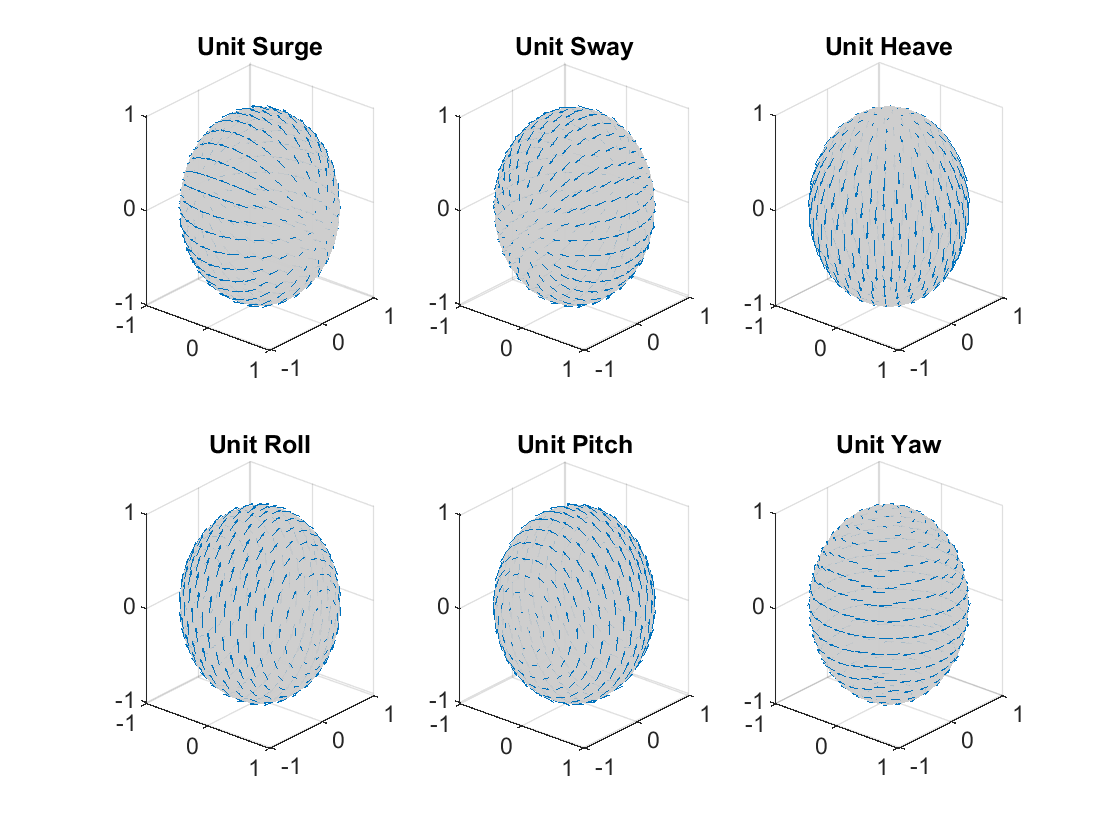
\includegraphics[width=.6\linewidth]{Figures/Unit_Movement}
        \caption{Write something here}
        \label{fig:Unit_Movement}
    \end{center}
\end{figure}

\subsection{Camera Calibration}\label{sec:Background_cameraCal} %TODO: Pretty good, get someone to read
Computer vision begins with the camera detecting light from a scene. This light has travelled from its source, reflecting from an object, through the camera lens, and is recorded on the image sensor. For these rays of light that make up an image to be useful for representing the real-world, the geometry that transforms these rays from the three-dimensional real world to a two-dimensional image plane must be understood; i.e. the transformation from world coordinates to image coordinates.

The camera calibration process describes the camera with two sets of parameters, namely the intrinsic parameters, and the extrinsic parameters. The intrinsic parameters describe the geometric relationship between the camera model and its projection. And the extrinsic parameters describe the location and orientation or pose, of the camera with respect to the world frame.

This project uses a GoPro Hero 7 to test and verify the calibration routine. This section will cover camera models and outline why a planar model is used for the GoPro. It covers the mathematical tools used to capture the different effects that make our camera imperfect for representing the real world, and how these deviations can be corrercted.
\subsubsection{Camera Models}
The most elementary way of representing a camera is with the pinhole model. Light enters the aperture (pinhole) after reflecting from objects in a scene. For an ideal pinhole camera, only one ray enters the aperture from any point in the scene. The light is then projected onto a surface behind the aperture resulting in an image of the scene that is scaled proportionally to the focal length $f$.

\begin{figure}[ht]
    \begin{center}
        \includegraphics[width=.8\linewidth]{Figures/Pinhole_model}
        \caption{Elementary pinhole model of a camera: In practice, the appeture must be big enough to let light in, allowing a narrow ray of light from each point in the scene blurring the image. Therefore there is a tradeoff between brightness and sharpness.}
        \label{fig:PinholeModel}
    \end{center}
\end{figure}

\Cref{fig:PinholeModel} shows an ideal pinhole camera model and its parameters, where $f$ is the focal length, $Z$ is the distance along the optical axis to an object, $x$ is the size of the projected object and $X$ is the size of the object. For this model, \eqref{eq:pinholeEQ} is the relationship between the projected image and the object
\begin{equation}\label{eq:pinholeEQ}
	\frac{-x}{f} = \frac{X}{Z}
\end{equation}
Due to how light enters the camera, the image projection from a pinhole model is projected upside down. This issue is fixed in a planar camera model. The planar model is similar to a pinhole model, however rather than passing through an aperture, light travels from each point in the scene, intersects the image plane and converges to a single point known as the \textit{centre of projection} \Cref{fig:PlainarModel}. The Plainar Model better represents the geometry of a camera with a lens, albeit a camera with an impossibly perfect lens.

\begin{figure}[ht]
	\begin{minipage}[c]{0.3\linewidth}
		\centering
		\begin{tabular}{l l}
			$C$ &: Centre of projection\\
			$\{c\}$ &: Camera co-ordinates\\
			$P$ &: Point in world space\\
			$P'$ &: Point on image plane\\
			$\vec{u}, \vec{v}$ &: Image co-ordinates\\
			$f$ &: Focal length\\
			$I$ &: Image plane
		\end{tabular}
	\end{minipage}
	\begin{minipage}[c]{0.65\linewidth}
		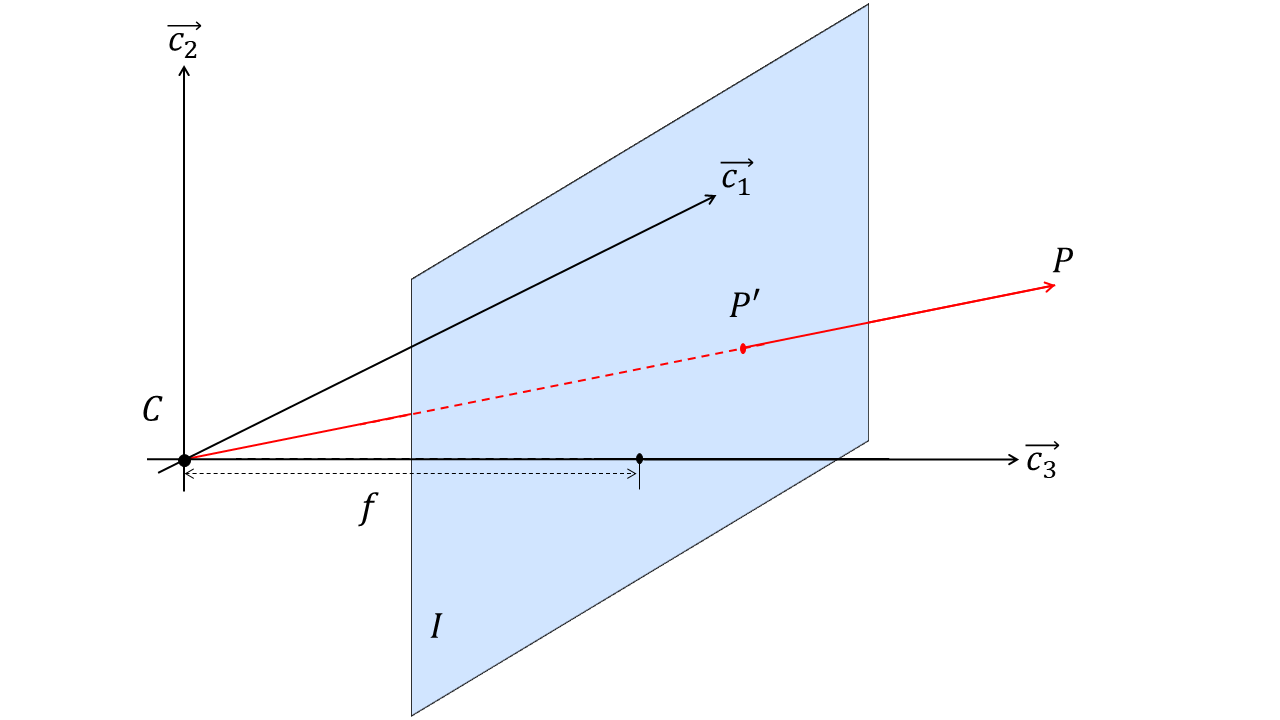
\includegraphics[width=1\linewidth]{Figures/Planar_Model}	
	\end{minipage}
\caption{Ideal camera model. A point $P$ in camera coordinates $(c_{1}, c_{2}, c_{3})$ is projected and displayed as a point $p$ in image co-ordinates $(u, v)$}
\label{fig:PlainarModel}
\end{figure}
The idea behind modelling and calibrating a camera is to identify and cancel out imperfections caused by slight defects in the manufacturing process. Firstly, the image sensor is often mounted out of line from the optical centre of the lens. Therefore, the parameters $u_{0}$ and $v_{0}$ are introduced to model this displacement from the optical centre. Furthermore, each pixel is not necessarily square, causing a small discrepancy between the focal length in the $u$ and $v$ directions. These discrepancy are captured in the $f_{u}$ and $f_{v}$ parameters. The following \Cref{eq:ProjectionEquations} project a point $P_{c_{1}, c_{2}, c_{3}}$ to image sensor co-ordinates $(u, v)$:
\begin{equation}\label{eq:ProjectionEquations}
	\begin{split}
		u = &f_{u} \times \frac{c_{1}}{c_{3}} + u_{0}\\
		v = &f_{v} \times \frac{c_{2}}{c_{3}} + v_{0}
	\end{split}
\end{equation}
\subsubsection{Projective Geometry}
Projective geometry is a tool describing the relationship that transforms a point from world coordinates $(n_1, n_2, n_3)$ into image coordinates $(u, v)$. When applying such transformations, it is convenient to add an extra dimension to each vector in the transform. for instance, a point that lies in a $n$ dimensional space is represented as a $n+1$ dimensional vector. this coordinate system is known as \textit{homogeneous coordinates}. for example, a point lying on a plane at $(x, y)$ is represented by the homogeneous coordinates $(x, y, z)$. It is important to note that in homogeneous coordinates, any two vectors that share a common factor represents the same point in Euclidean geometry. This has the effect that a point in Euclidean geometry can be represented by an infinite number of homogeneous vectors. for instance $\alpha * (q_{1}, q_{2}, q_{3}) \equiv (q_{1}, q_{2}, q_{3})$. The original primitive point is recovered by dividing through by $q_{3}$.

the utility of homogenious coordinates becomes clear when common transformations such as translation, rotation and scailing are attempted in . Homogenious coordinates allow these transformations to be implemented with matrix opperations. This is how projective geometry allows the camera intrinsic parameters $f_{u}, f_{v}, u_{0}, v_{0}$ to be arranges into a single $3\times3$ \textit{camera intrinsic matrix} matrix. Bringing all of thees concepts together, the \Cref{eq:ProjectionEquations} can be implemented as a single martix opperation of the form:

\begin{equation}
	p = \mathbf{M}\mathbf{r}^{C}_{P/C}
\end{equation}
where:
\begin{equation}\label{eq:CameraMatrix}
	P = 
    \begin{bmatrix}
        u\\
        v\\
        w
	\end{bmatrix},
	M = 
	\begin{bmatrix}
        f_{u} & 0 & u_{0}\\
        0 & f_{v} & v_{0}\\
        0 & 0 &1
	\end{bmatrix}
	\textrm{and } \mathbf{r}^{C}_{P/C} = 
	\begin{bmatrix}
        c^{c}_{1}\\
        c^{c}_{2}\\
        c^{c}_{3}
	\end{bmatrix}
\end{equation}
Some older camera manufacturing processes produce nonrectangular image sensors, i.e. they produced parallelogram shaped sensors. To account for this, a final \textit{skew} parameter was included. Most modern cameras are produced with close to no skew therefor the error that this effect causes is below the noise floor and assumed to be $0$.
\subsubsection{Lens Distortion}
The optics inside a camera are yet another source of error in an image. Similar to correcting for the cameras geometry (captured in \ref{eq:CameraMatrix}), lens distortion must be accounted for. The leading method for correcting Lens distortion uses a \textit{Brown-Conrady model} from \cite{fryer1986lens}. This model characterises the two most prominent sources of distortion, naimley \textit{radianl distortion} and \textit{tangental distortion} and undistorts the image pixel locations.

In an ideal camera, the lense would take the shape of a perfect paraboloid. However it is much easier and cheeper to produce a sperical lens. The spherical shape of the lens tends to "over bend" rays entering farther from the optical center producing the effect known as \textit{Radial Distortion} \cref{fig:RadialDistortion}. Typically a taylor series is used to characterise the distortion caused by the lens \cite{learningOpenCV}. This polynomial takes the form:
\begin{equation}
	f(r) = a_{0} + a_{1}r + a_{2}r + a_{3}r\dots
\end{equation}
where $r = \sqrt{u^{2} + v^{2}}$ is the radial distance from the optical centre.

\begin{figure}[ht]
	\subfloat[][Red - "spherical" lens

				Blue - paraboloidal lens]
				{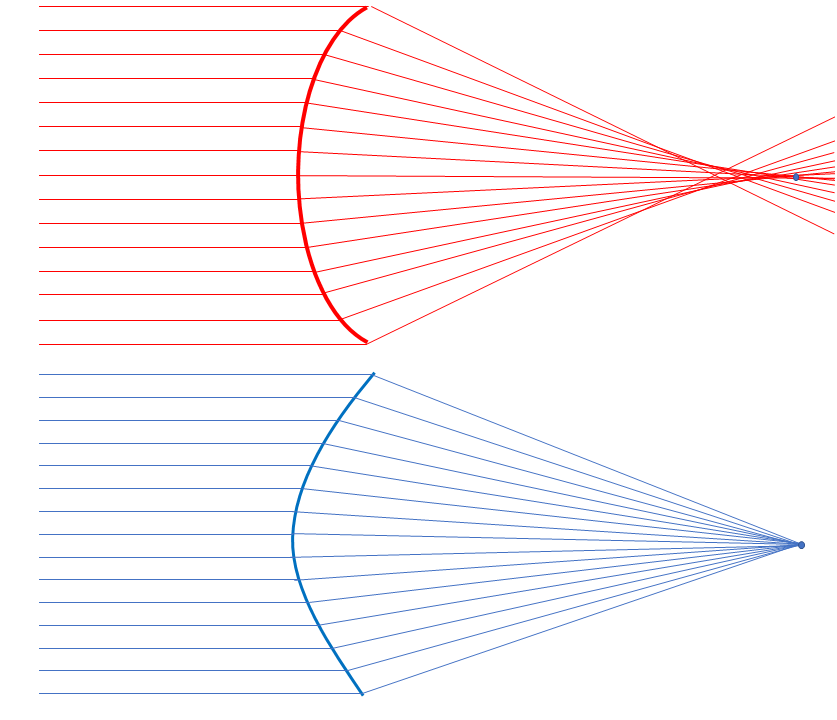
\includegraphics[width=.35\linewidth]{Figures/ParabolicLens}}
	\subfloat[Radial distortion is most clear on square objects]{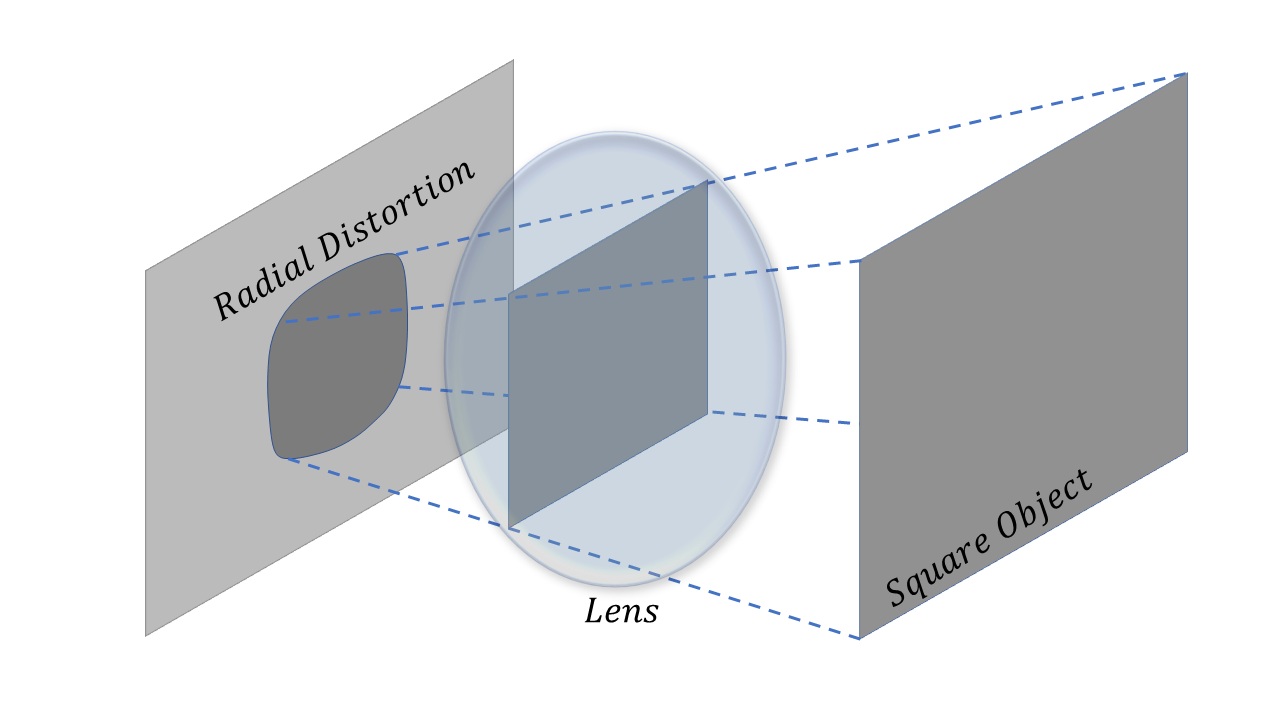
\includegraphics[width=.6\linewidth]{Figures/RadialDistortion}}
	\caption{Radial distortion also known as \textit{Barrel Distortion}. The farther from the centre a ray enters, the larger the barrel distortion bends it.}	
	\label{fig:RadialDistortion}
\end{figure}

However, for radial distortions, at the optical centre of the lense, deviation cause to the light rays is minimal i.e. $f(r) = 0$ at $r = 0$. This further implies that $a_0 = 0$. Additionally, becaues the distortion must be symetrical in $r$, the coefficents of the odd powers of $r$ equal $0$. This means that only the parameters needed for radial distortion correction are the coefficents of even powers of $r$ \cite{learningOpenCV}. Typically, no more than three radial distortion parameters $(k_{1}, k_{2}, k_{3})$ are needed. However, for high \textit{field of view} cameras, upto $K_{6}$ may be necessary. Once these parameters are found, each pixel will be rescaled according to the following equations:
\begin{equation}\label{eq:radialParameters}
	\begin{split}
	u' = u\times(1+k_{1}r^{2} + k_{2}r^{4} + k_{3}r^{6})\\
	v' = v\times(1+k_{1}r^{2} + k_{2}r^{4} + k_{3}r^{6})
	\end{split}
\end{equation}
where $u'$ and $v'$ are the undistorted pixel coordinates.

Not only is it expensive and dificult to produce a lens that perfectly trains rays of light onto the \textit{centre of projection} of a camera, it is also dificult to mechanically mount the image sensor to the camera body such that it is parallel to the lense.

\begin{figure}[ht]
	\subfloat[Ray diagram of tangental distortion]{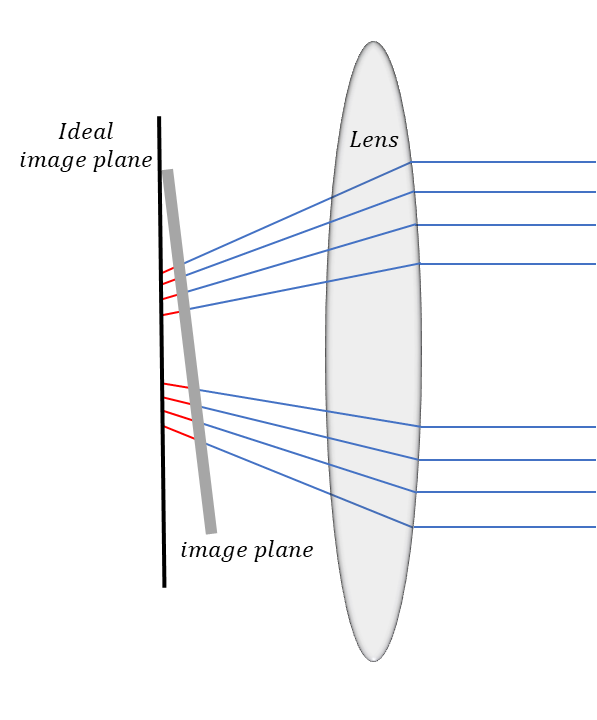
\includegraphics[width=.4\linewidth]{Figures/tangentalDistortion}}
	\subfloat[Tangental distortion of a flat grid]{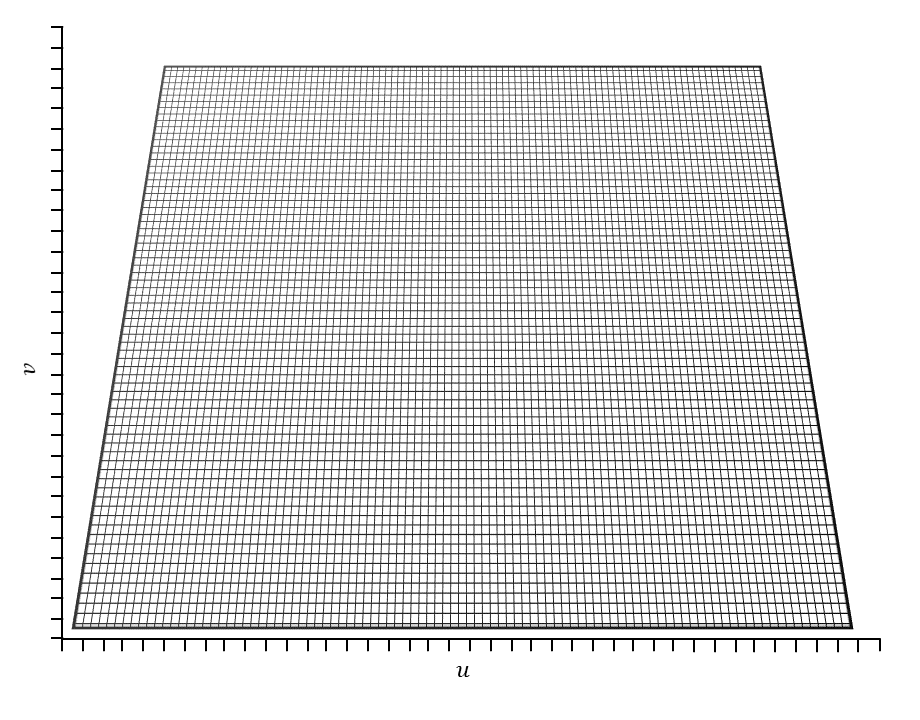
\includegraphics[width=.6\linewidth]{Figures/tangentalImage}}
	\caption{Extream example of tangental distortion.}	
	\label{fig:RadialDistortion}
\end{figure}

Two additional parameters $p_{1}$ and $p_{2}$ are introduced to minimally characterise this tangental distortion such that:

\begin{equation}\label{eq:tangentalParameters}
	\begin{split}
		u' &= u + [2p_{1}uv + p_{2}(r^{2} + 2u^{2})]\\
		v' &= v  + [p1(r^{2} + 2v^2) + 2p_{2}uv]
	\end{split}
\end{equation}
There are many other aspects within an average camera that cause image distortion, howerver these effects contribute a minor amount to the accuracy of measurements from an image so for this project will be assumed $0$. Both Matlab and Open CV based camera calibration rotines are implemented and evaluated in this project. The camera calibration routine for Matlab \textit{estimateCameraParameters();} returns an object containing the camera matrix \ref{eq:CameraMatrix}, radial distortion parameters \ref{eq:radialParameters} and tangental distortion parameters \ref{eq:tangentalParameters}, along with information about the calibration photos. When using \textit{Open CV}, these parametetrs are packaged into a \textit{distortion vector}. For this project, six radial distortion parameters were used to capture the distortion for a Go Pro Hero 7. Therefor the distortion vector from Open CV is organised as $(k_{1}, k_{2}, p_{2}, p_{1}, k_{3}, k_{4}, k_{5}, k_{6})$.
From \cref{eq:radialParameters} and \cref{eq:tangentalParameters}, the \textit{Brown-Conrady model} is as follows:
\begin{equation}
	\begin{split}
		u' &= u\left(\frac{1  +k_{1}r^{2} + k_{2}r^{4} + k_{3}r^{6}}{k_{4}r^{2} + k_{5}r^{4} + k_{6}r^{6}}\right) + 2p_{1}uv + p_{2}(r^{2} + 2u^{2})\\
		v' &= v\left(\frac{1  +k_{1}r^{2} + k_{2}r^{4} + k_{3}r^{6}}{k_{4}r^{2} + k_{5}r^{4} + k_{6}r^{6}}\right)  + p_{1}(r^{2} + 2v^{2}) + 2p_{2}uv\\
	\end{split}
\end{equation}
Now that the camera can be described mathematically through the intrinsic parameters and distortion parameters, pixel location in the image can be \textit{undistorted}. \Cref{fig:DistortionMovement} shows the movement of a subset of pixels from a GoPro Hero 7 image. Notice the movement of pixels in the centre of the image move far less than those further away radially.
\begin{figure}[ht]
    \begin{center}
        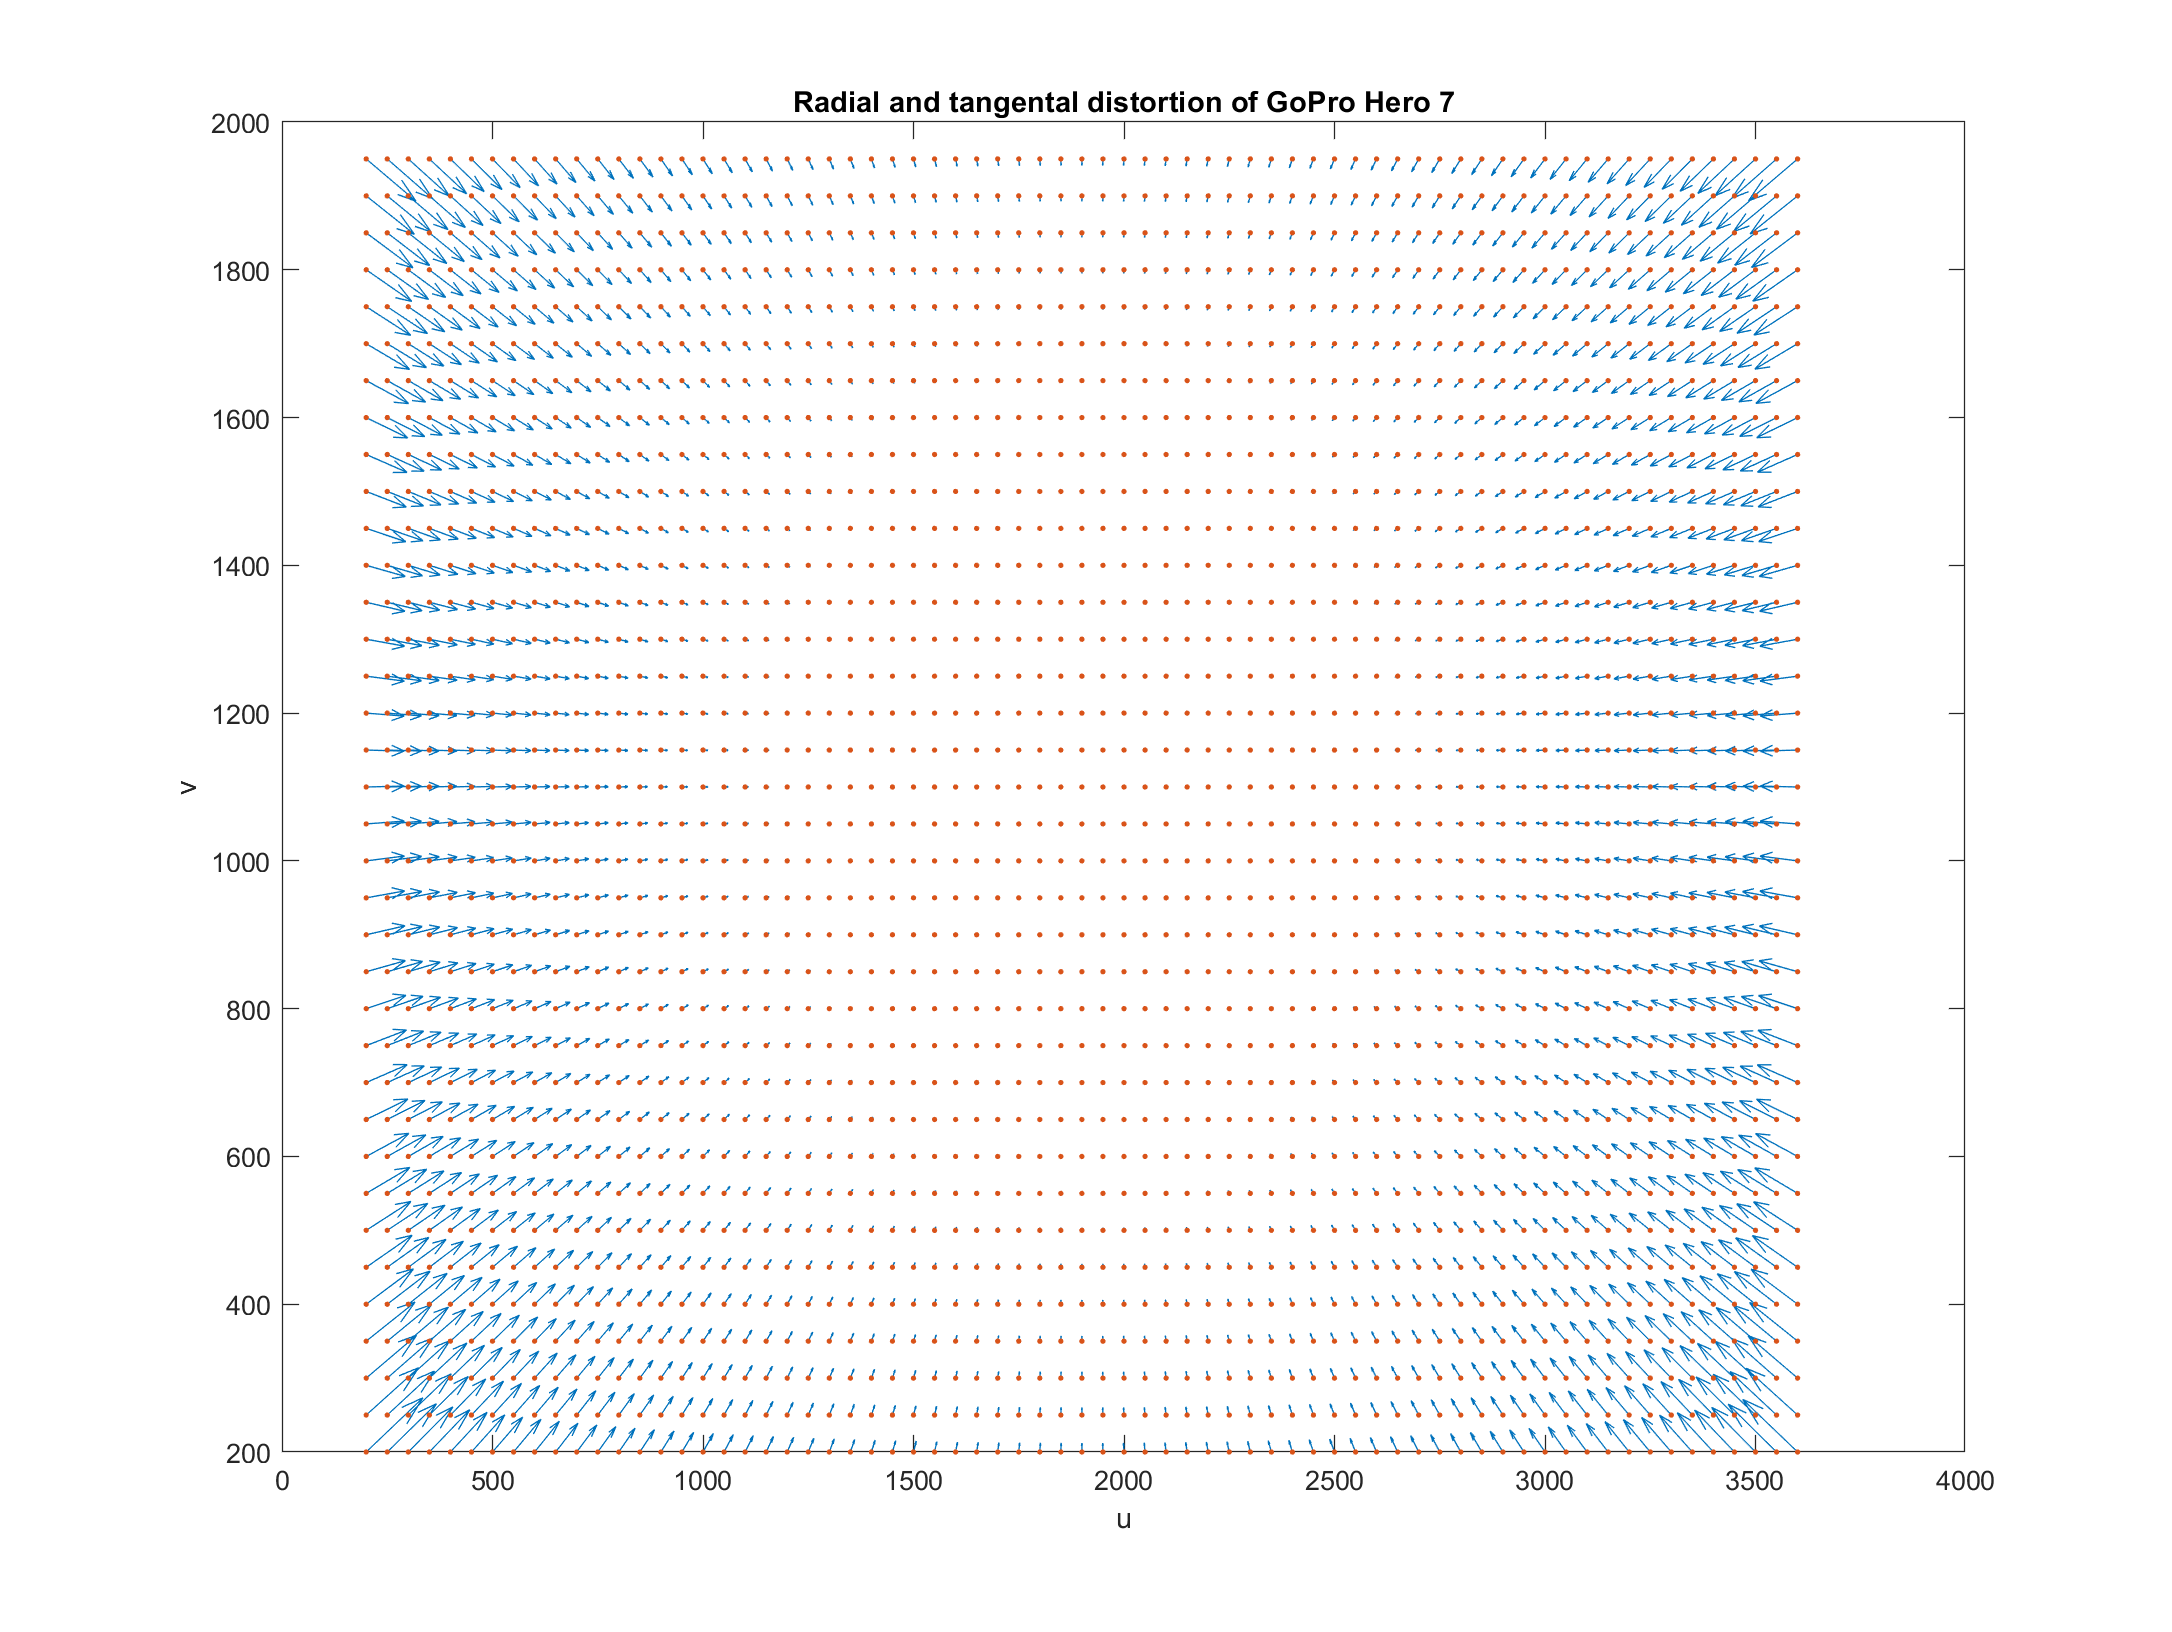
\includegraphics[width=.9\linewidth]{Figures/Matlab/DistortionMovement}
        \caption{Shows the movement of a sample of pixels based on the parameters of a GoPro}
        \label{fig:DistortionMovement}
    \end{center}
\end{figure}

%%%%%%%%%%%%%%%%%%%%%%%%%%%%%%%
\newpage
\section{Simulation in Unity}
Unity 3D game engine was used to create the simulation for collecting the data required to develop and test an obstacle avoidance algorithm. This game engine was a convenient way to create an environment that could obtain a ground truth dataset and real world data could be evaluated against.

In order to utelise the Unity engine as a simulation platform, the behavior of the rover needed to be defined. This was done by implementing basic aerodynamics into the movement of the rover. \Cref{lst:AircraftMovement} shows the equations that dictated the rovers movement about the environment.

\begin{lstlisting}[
    language=C,
	float=h,
	numbers=none,
    xleftmargin=1cm,
    frame=shadowbox,
	caption={A simple aerodynamic lift caculation that aproximates the movement of the rover}
	\label{lst:AircraftMovement}
	]
private void calculateLift ()
{
	Vector3 vel = rb.velocity;
	Vector3 localVel = transform.InverseTransformDirection(vel);
	Vector3 dragDirection   = -rb.velocity.normalized;
	Vector3 thrustDirection = transform.forward;
	Vector3 liftDirection   = Vector3.Cross(-dragDirection, transform.right);

	float angleOfAttack   = Mathf.Atan2(-localVel.y, localVel.z);
	float liftCoeff = lc0 + 2*Mathf.PI*angleOfAttack;
	float drag = (0.5f) * Mathf.Abs(roh) * Mathf.Abs(dragCoeff) * vel.sqrMagnitude;
	float lift = (0.5f) * Mathf.Abs(roh) * liftCoeff * vel.sqrMagnitude;

	rb.AddForce(thrustDirection * thrust);
	rb.addforce(dragdirection * drag);
	rb.AddForce(liftDirection * lift);
}
\end{lstlisting}

Furthermore, control actions were also calculated allowing the rover to be interacted with. For testing purposes these control actions were tied to the \textbf{W}, \textbf{A}, \textbf{S}, \textbf{D} keys, allowing the tester to apply control torques to the rover during simulation. The function that applies these torques can be seen in \cref{lst:calculateControlTorque}

\begin{lstlisting}[
    language=C,
	float=h,
	numbers=none,
    xleftmargin=1cm,
    frame=shadowbox,
	caption={Adds the demanded control torques to the simulated aircraft}
	\label{lst:calculateControlTorque}
	]
void calculateControlTorque() {
	Vector3 vel = rb.velocity;
	Vector3 localVel = transform.InverseTransformDirection(vel);

	float elevatorTorque = (elevatorD - elevatorU);
	float aileronTorque = (AileronL - AileronR);
	float rudderTorque = (rudderR - rudderL);

	rb.AddTorque(transform.right * elevatorTorque);
	rb.AddTorque(transform.forward * aileronTorque);
	rb.AddTorque(transform.up * rudderTorque);
}
\end{lstlisting}

By utelising the in built physics engine of unity, velocity of the rover was able to be accurately and efficiently extracted from the scene. Both the lift Calculationd and the data was recorded within the \textbf{FixedUpdate()} function. This function is built in to unity, and allows processes to be run at exatly $30$ frames per second. This is the function that accomodates all of the force calculations, in order to maintain a fixed timestep between adding forces to the sumulated rover.

Depth information from the simulated environment is extracted using raycasts. Typically used for hit detection in shooter games, the \textbf{Physics.Raycast()} function projects a ray into the scene in a defined direction and intersects an object in the scene. Depth can then be recovered from the origen of the ray to the object it has intersected with. The raycast functionality of the Unity engine was utelised by first defining a set of direction vectors along which The depth of the environment could be calculated. These direction vectors were created by itterating through a double for loop that calculated discretised euler angels of a sphere. The calculatins for the raycast direction vectors are seen in \cref{lst:raycastSphere}

\begin{lstlisting}[
    language=C,
	float=h,
	numbers=none,
    xleftmargin=1cm,
    frame=shadowbox,
	caption={Direction Vectors that define the euler angles for each raycast}
	\label{lst:raycastSphere}
	]
for (int ii = 1; ii < rX; ii++)
{
	for (int jj = 1; jj < rY; jj++)
	{
		float theta = jj * ((fovY) / (rY)) - fovY/2;
		float phi   = ii * ((fovX) / (rX)) + (Mathf.PI / 2 - fovX / 2);

		dir[ii, jj].x = Mathf.Cos(theta) * Mathf.Cos(phi);
		dir[ii, jj].z = Mathf.Cos(theta) * Mathf.Sin(phi);
		dir[ii, jj].y = -Mathf.Sin(theta);
	}
}
\end{lstlisting}
Where \textbf{fovX} and \textbf{fovY} define the $x, y$ field of view and where \textbf{rX} and \textbf{rY} define $x, y$ resoulution for the simulated camera. 
%%%%%%%%%%%%%%%%%%%%%%%%%%%%%%%
\newpage
\section{Optical Flow - Simulation}
After gathering the 

\begin{figure}[ht]
    \begin{center}
        \includegraphics[width=.6\linewidth]{Figures/SphericalFlowResultsExample}
        \caption{Write something here}
        \label{fig:Unit_Movement}
    \end{center}
\end{figure}

\subsection{Measurement Model}
\begin{figure}[ht]
    \begin{center}
        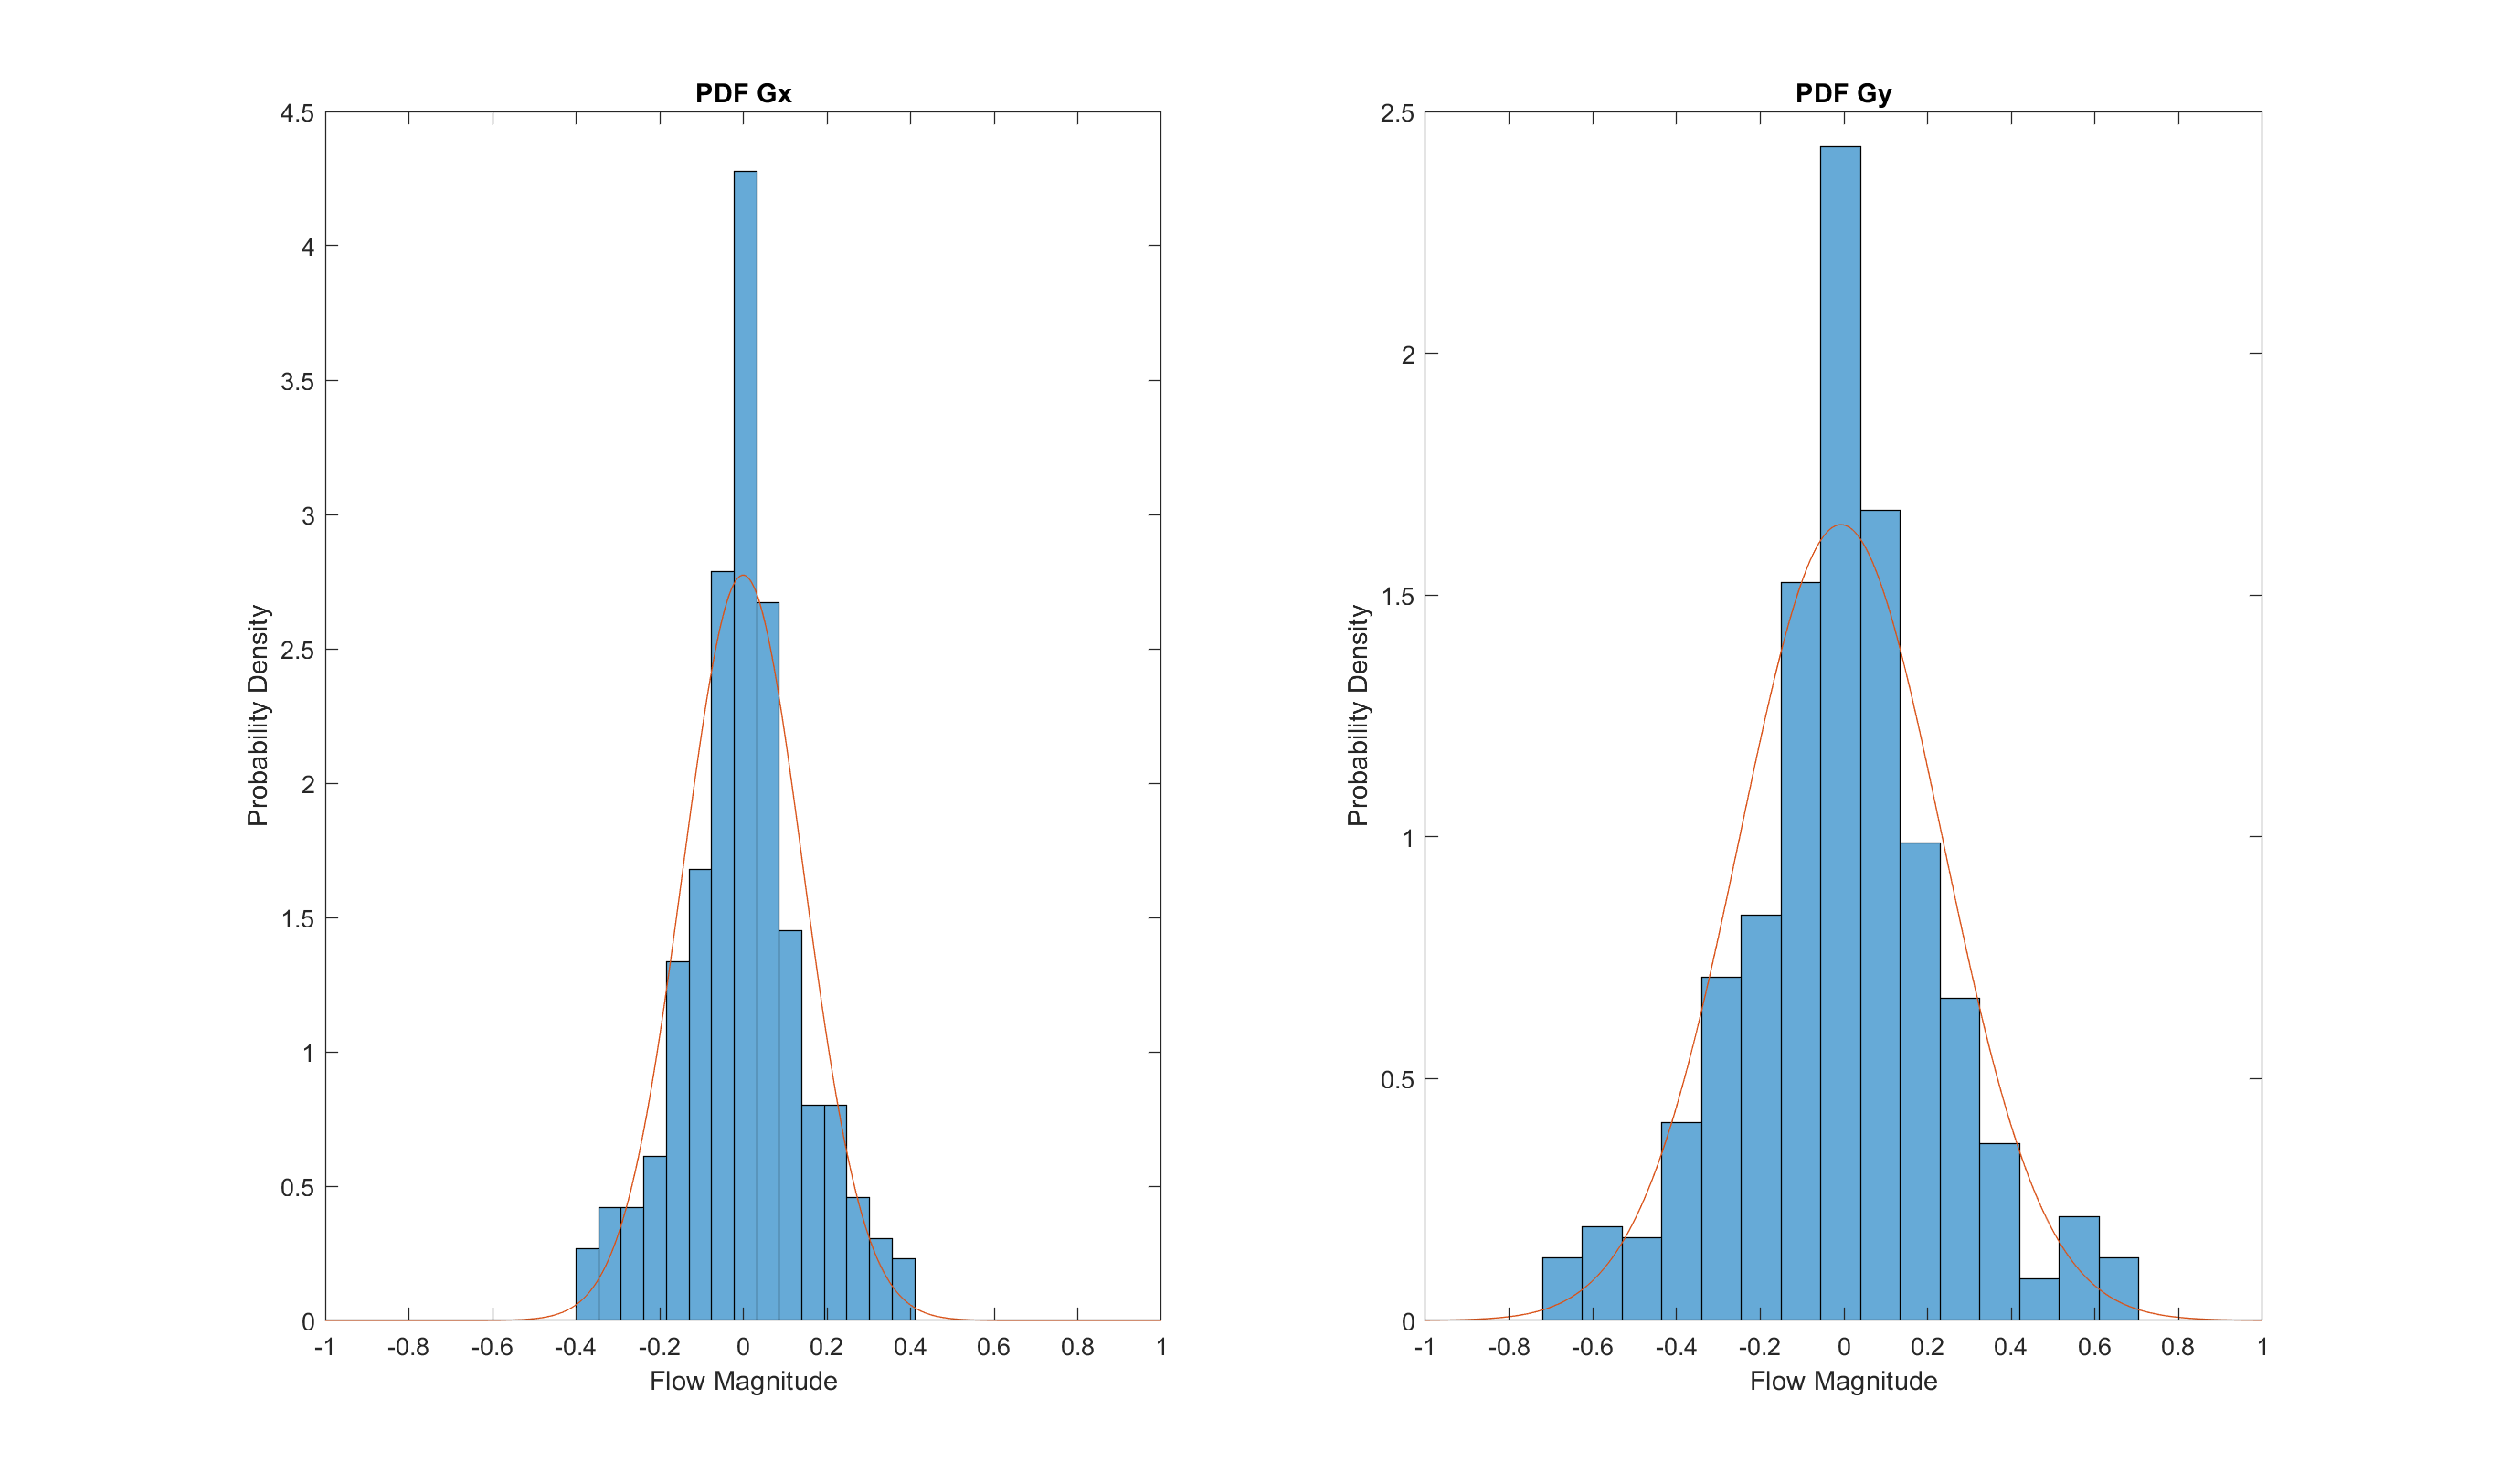
\includegraphics[width=.6\linewidth]{Figures/Matlab/GoPro_Noise_PDF}
        \caption{Write something here}
        \label{fig:GoPro_Noise_PDF}
    \end{center}
\end{figure}
\subsection{Farneback Algorithm - OpenCV}

\newpage
\section{Camera Calibration}
As discussed in \Cref{sec:Background_cameraCal} it is imperitive to understand and account for the construction and imperfections in a camera, if the measurments taken need to be relevent outside image coordinates. This section outlines the procedure used in this project to correct a GoPro hero 7 using a planar camera model and a 6th order equation to correct for distortion parameters.

\subsection{Calibration Boards}\label{sec:CalibrationBoards}
Theoretically, to calibrate a camera any object could be used as a calibration object, so log as it is appropriately characterised. However it is much more practical to use a well defined and easily measured object. For this reason, a flat rigid checker pattern was chosen. \Cref{fig:cornerLocations} shows a representation of the layout for the chosen calibration pattern, however the true pattern consisted of a $10 x 7$ checker grid. These are the measurement input into the calibration algorithm, allowing it to perform a \textit{projective transform} and recover the cameras intrinsic parametres and distortion parametres. For the actual calibration board used see \cref{app:calibrationBoard}

\begin{figure}[ht]
    \begin{center}
        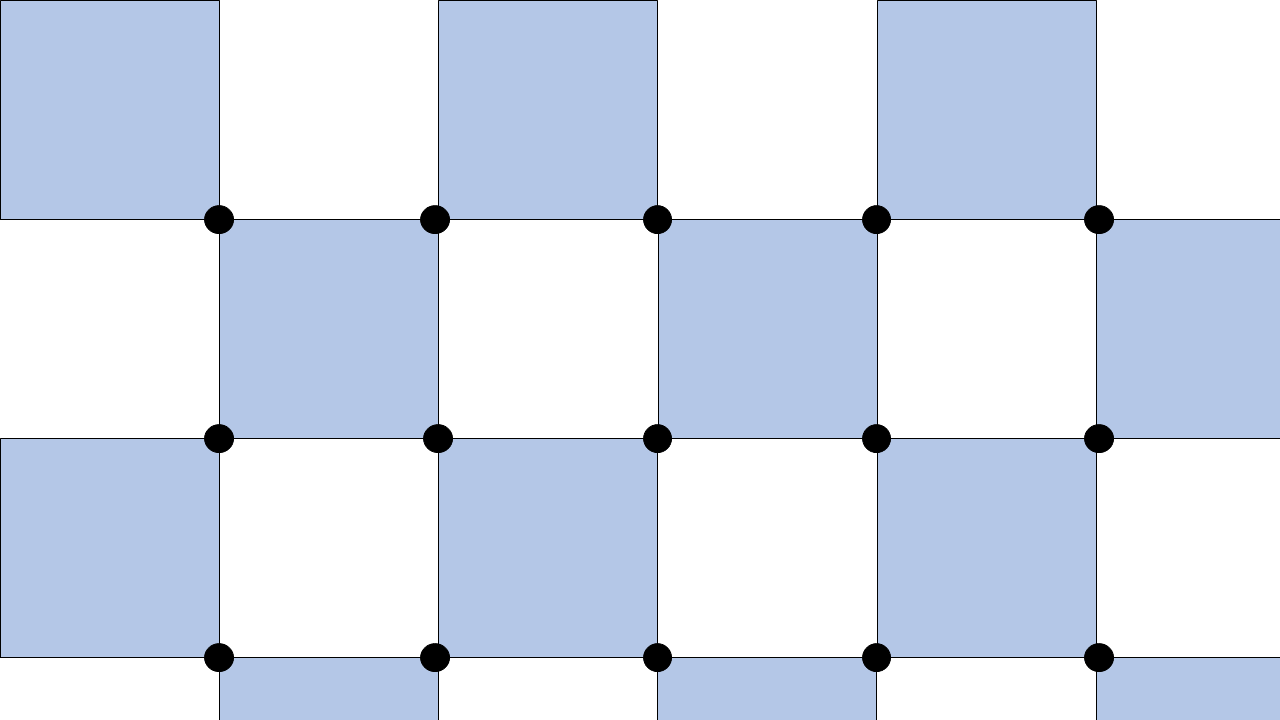
\includegraphics[width=.8\linewidth]{Figures/CalibCornerLocations}
        \caption{Expected corner locations for the purpose of camera calibration.}
        \label{fig:cornerLocations}
    \end{center}
\end{figure}

Now the calibration pattern has been defined, pictures of this pattern needed to be taken through the GoPro.In order to best capture the geometry of the camera, multiple views of the calibration board needed to be captured. Ensuring to capture shots of the calibration board in the edge of the image frame, as this is where the image can be most distorted. I found it most convenient to take a video of the pattern and later extracted the individual frames using \textit{ffmpeg}, a basic command line video processing tool.

Outlined in \cref{sec:Background_cameraCal}, the camera intrinsic parameters and distortion parameters are aproximated through a least squares fitting of the corner locations to the Brown-Conrady model. For this reason, multiple views of the calibration pattern are processed.

\subsection{Calibration Tool}
To calibrate the GoPro Hero 7 for in this project, A camera calibration tool was written in C\# using WPF as a graphical user interface(see \Cref{app:calibrationTool})). After extracting a collection of images from the calibration video as outlined in \cref{sec:CalibrationBoards}. These image are input into the calibration tool ready to be processed. The quality of the calibration images plays a large part in the resulting accuracy of the calibration routine. Using the calibration tool, the best frames from a list of frames can be selected to be calibrated against. An automatic function can also be chosen that selects 12 images with visable corners at random.

\subsection{Calibration Results}
For the purpose of evaluating the best tool for calibrating a camera, both the C\# openCV library and Mathlab's \textit{Vision Toolbox} were used. The calibration routine in Matlab


\begin{figure}[ht]
    \begin{center}
        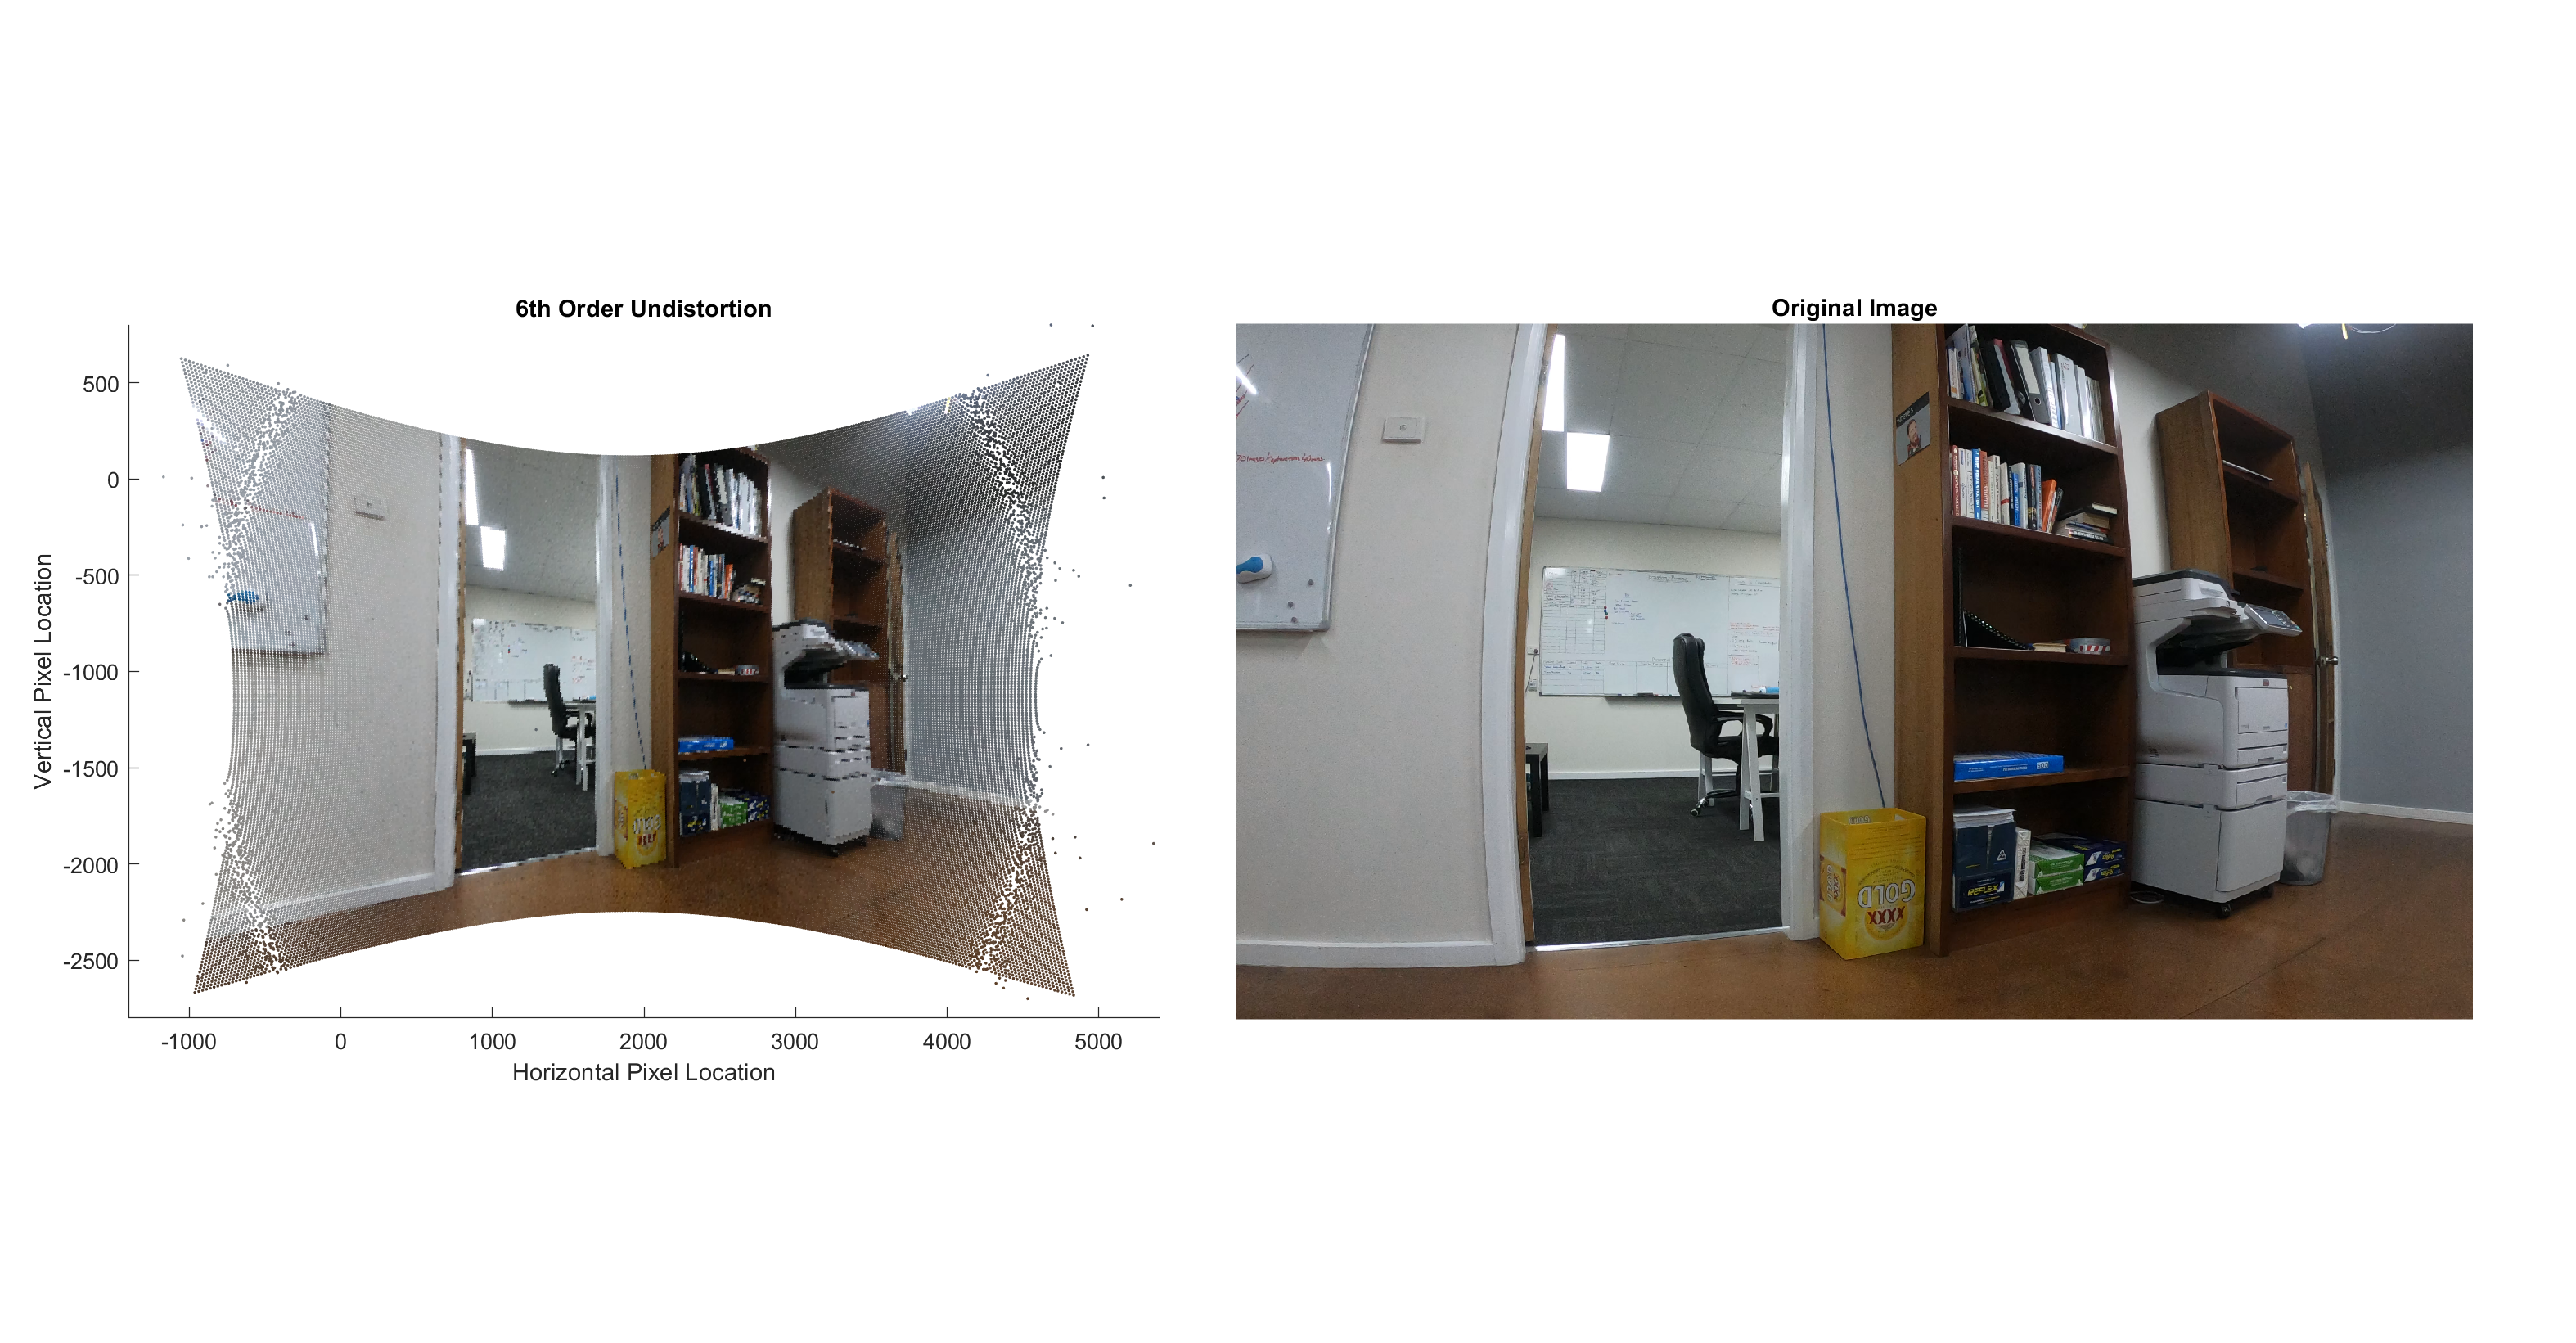
\includegraphics[width=.8\linewidth]{Figures/Matlab/6rdOrderUndistort}
        \caption{Caption}
        \label{fig:6rdOrderUndistort}
    \end{center}
\end{figure}
\begin{figure}[ht]
    \begin{center}
        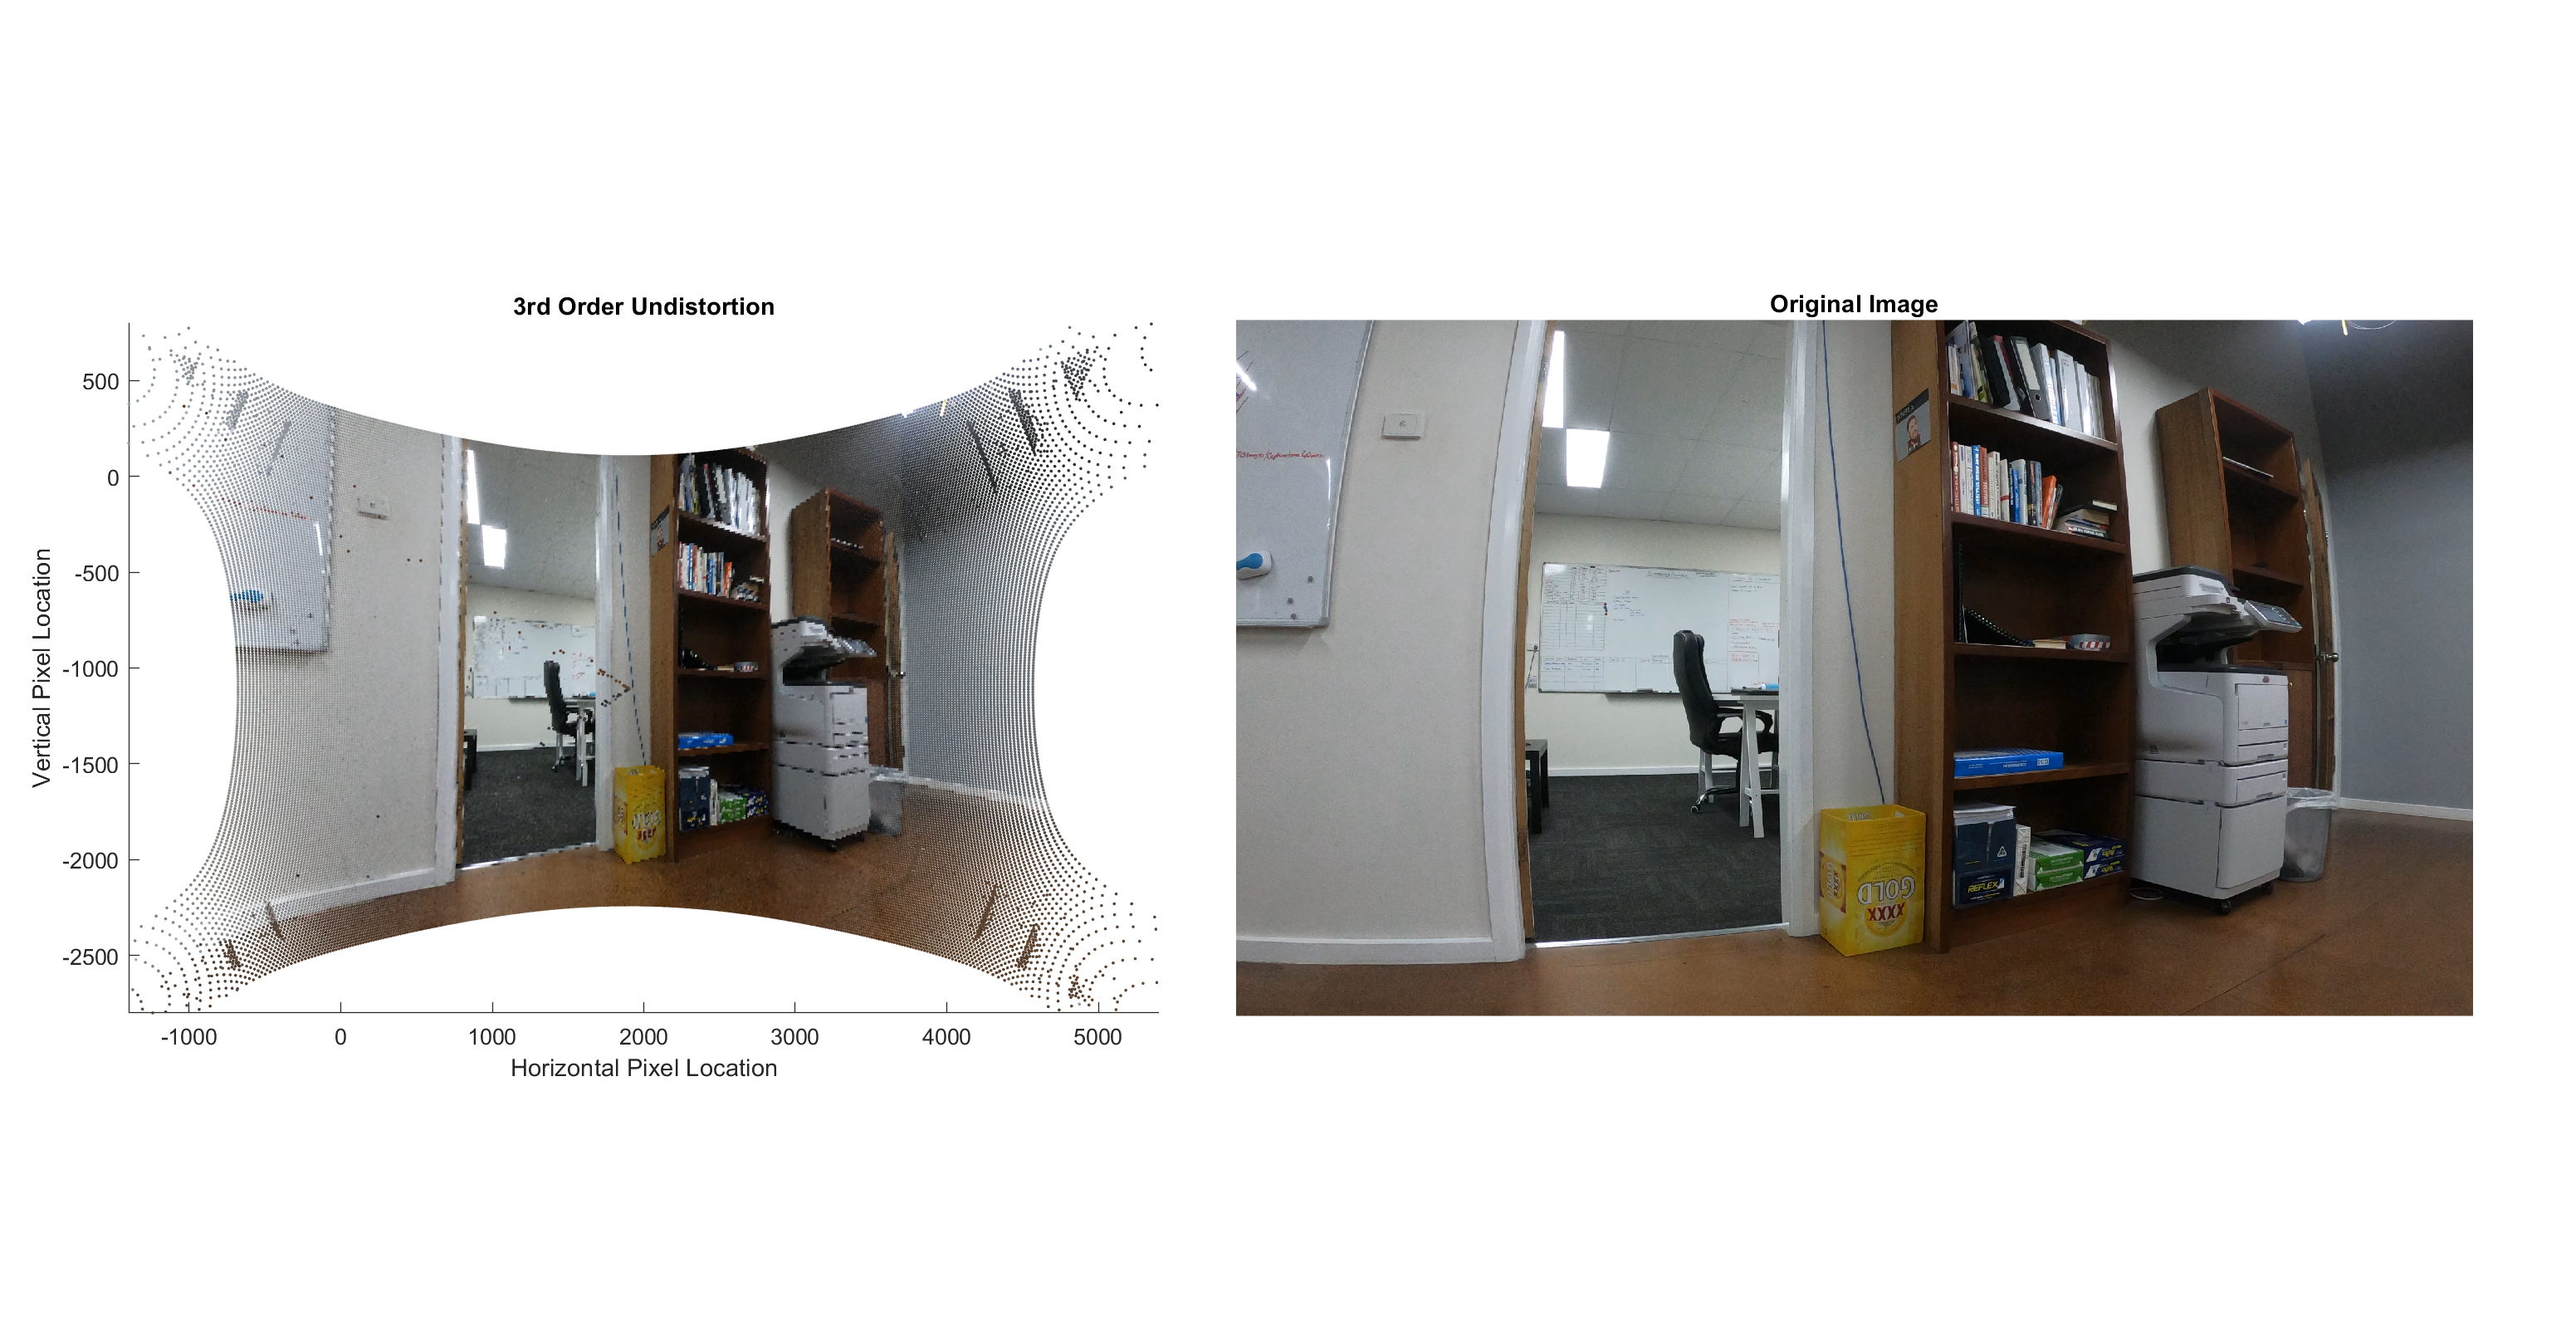
\includegraphics[width=.8\linewidth]{Figures/Matlab/3rdOrderUndistort}
        \caption{Caption}
        \label{fig:3rdOrderUndistort}
    \end{center}
\end{figure}
\begin{figure}[ht]
    \begin{center}
        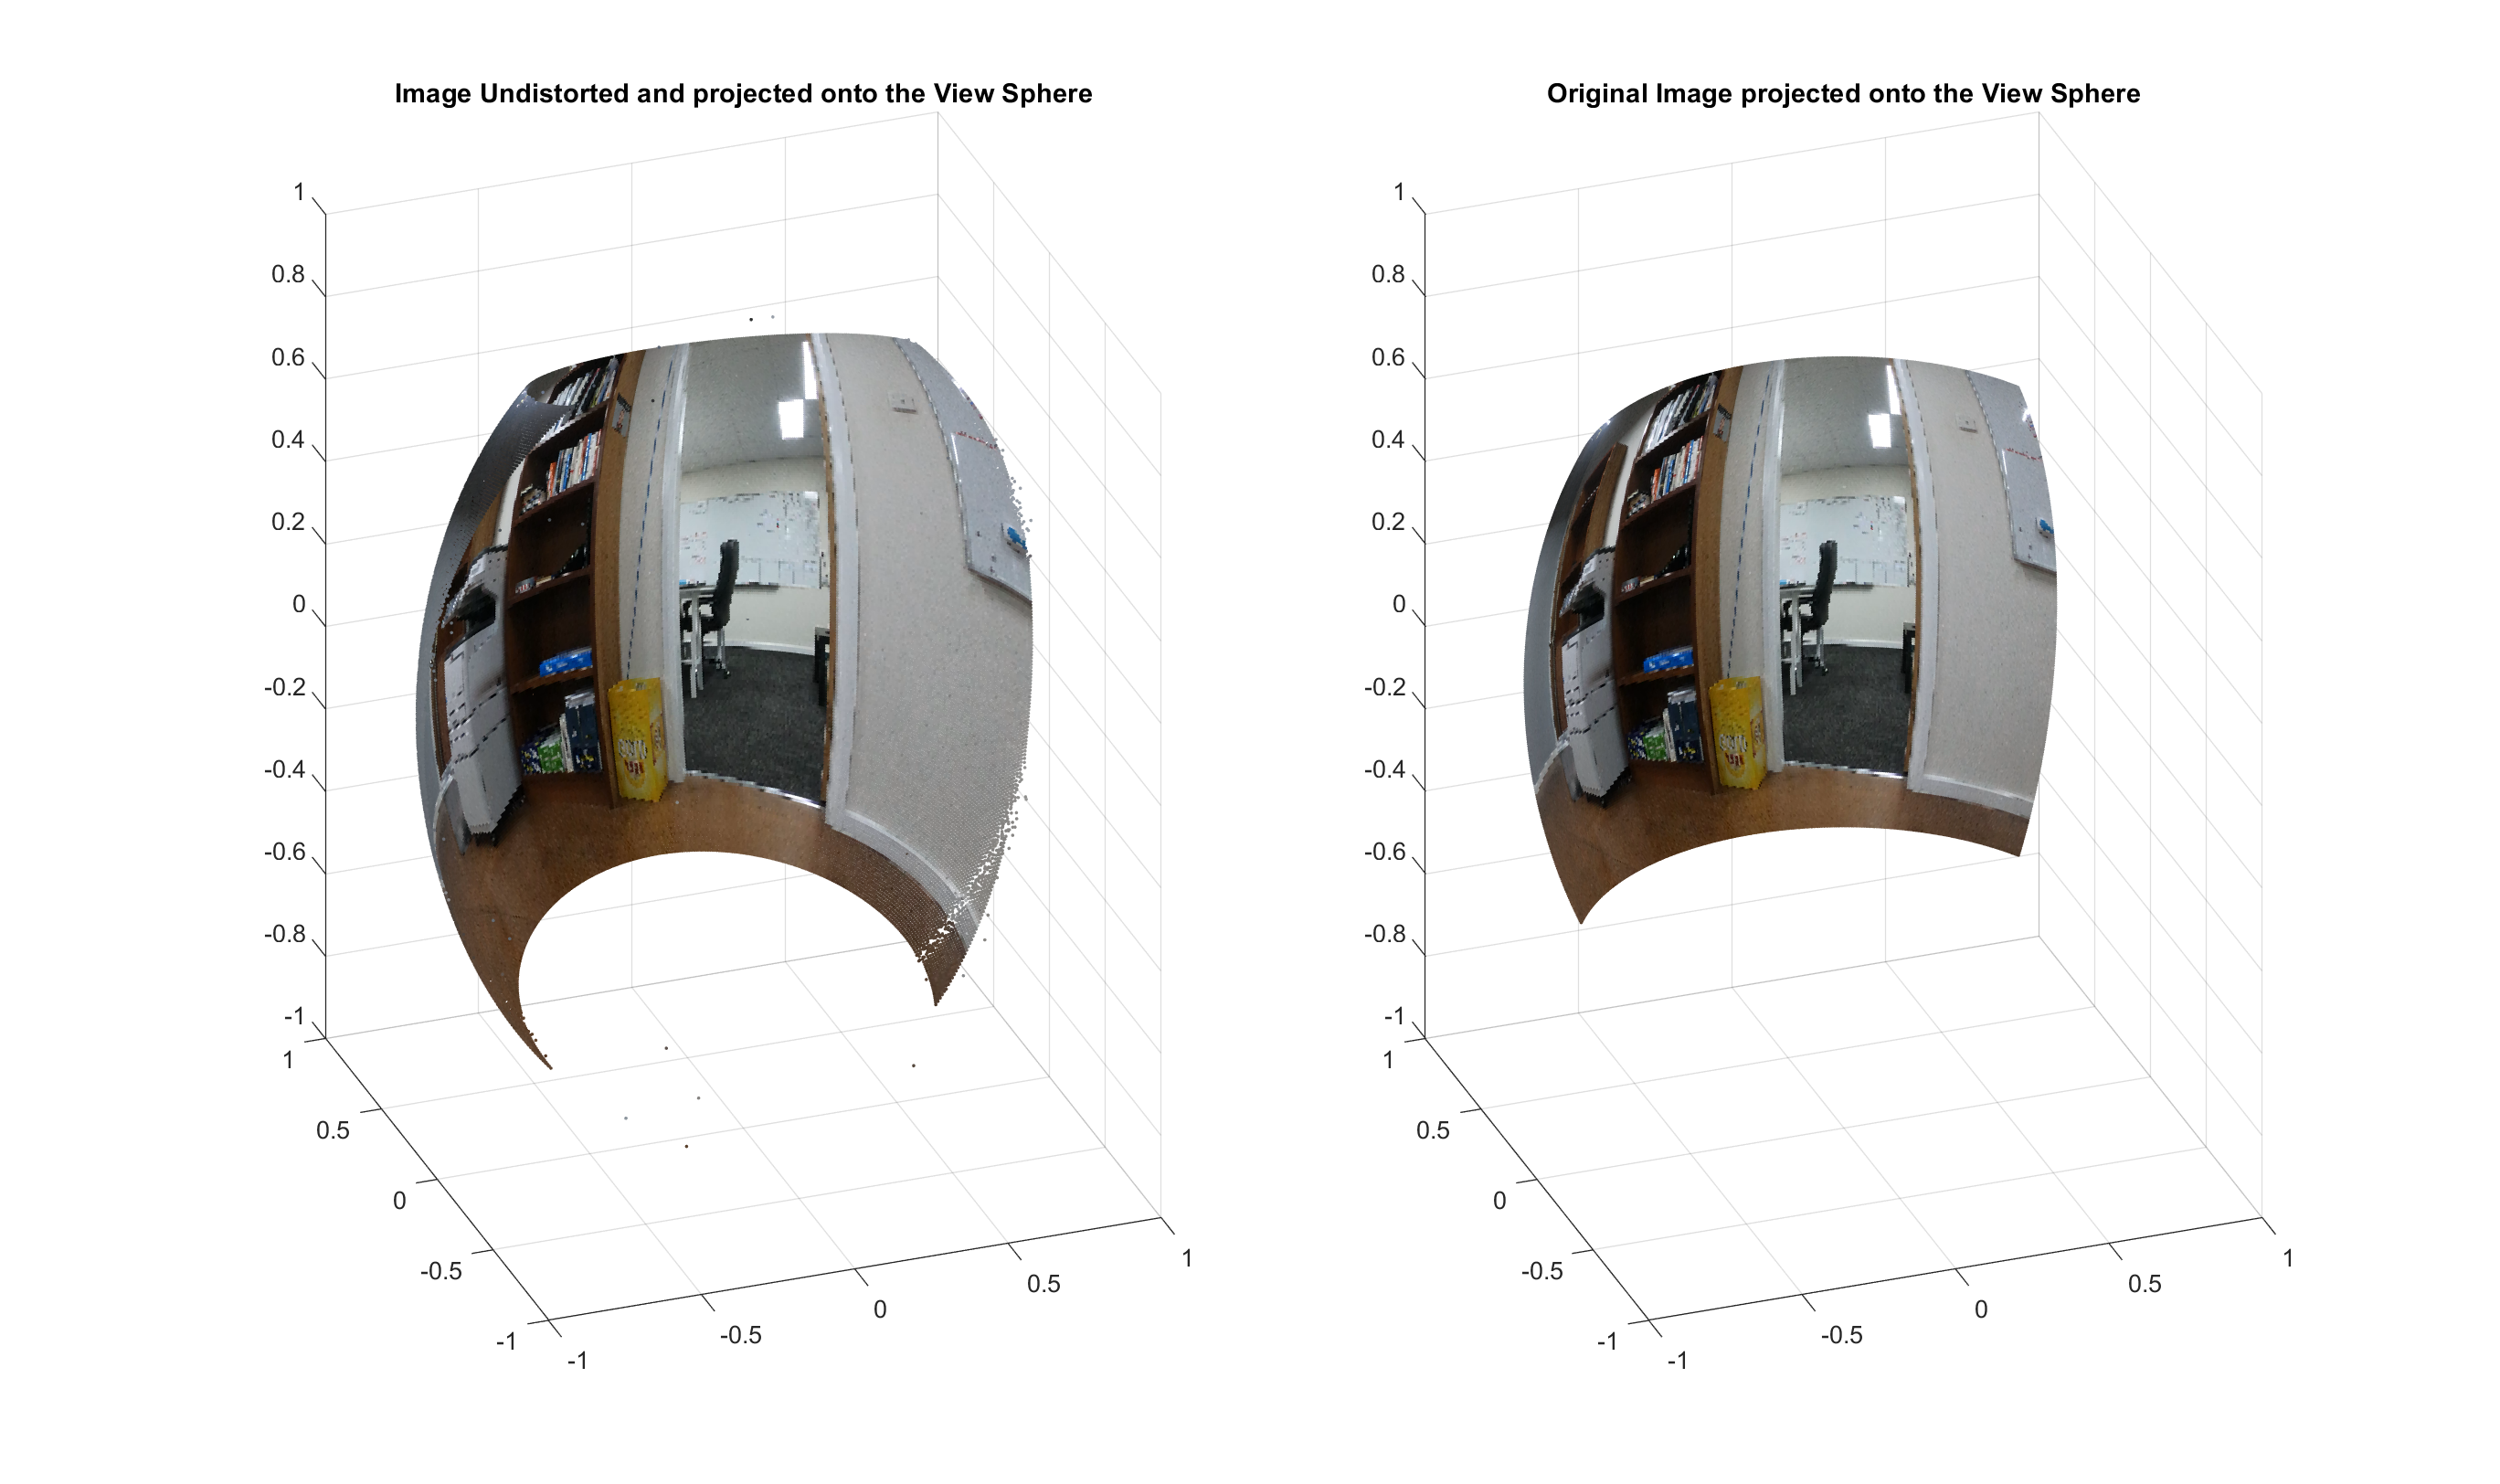
\includegraphics[width=.8\linewidth]{Figures/Matlab/Image_on_ViewSphere}
        \caption{Caption}
        \label{fig:Image_on_ViewSphere}
    \end{center}
\end{figure}
%%%%%%%%%%%%%%%%%%%%%%%%%%%%%%%
\newpage
\section{Vector Field Divergence for Object Avoidance}
\begin{figure}[ht]
    \begin{center}
        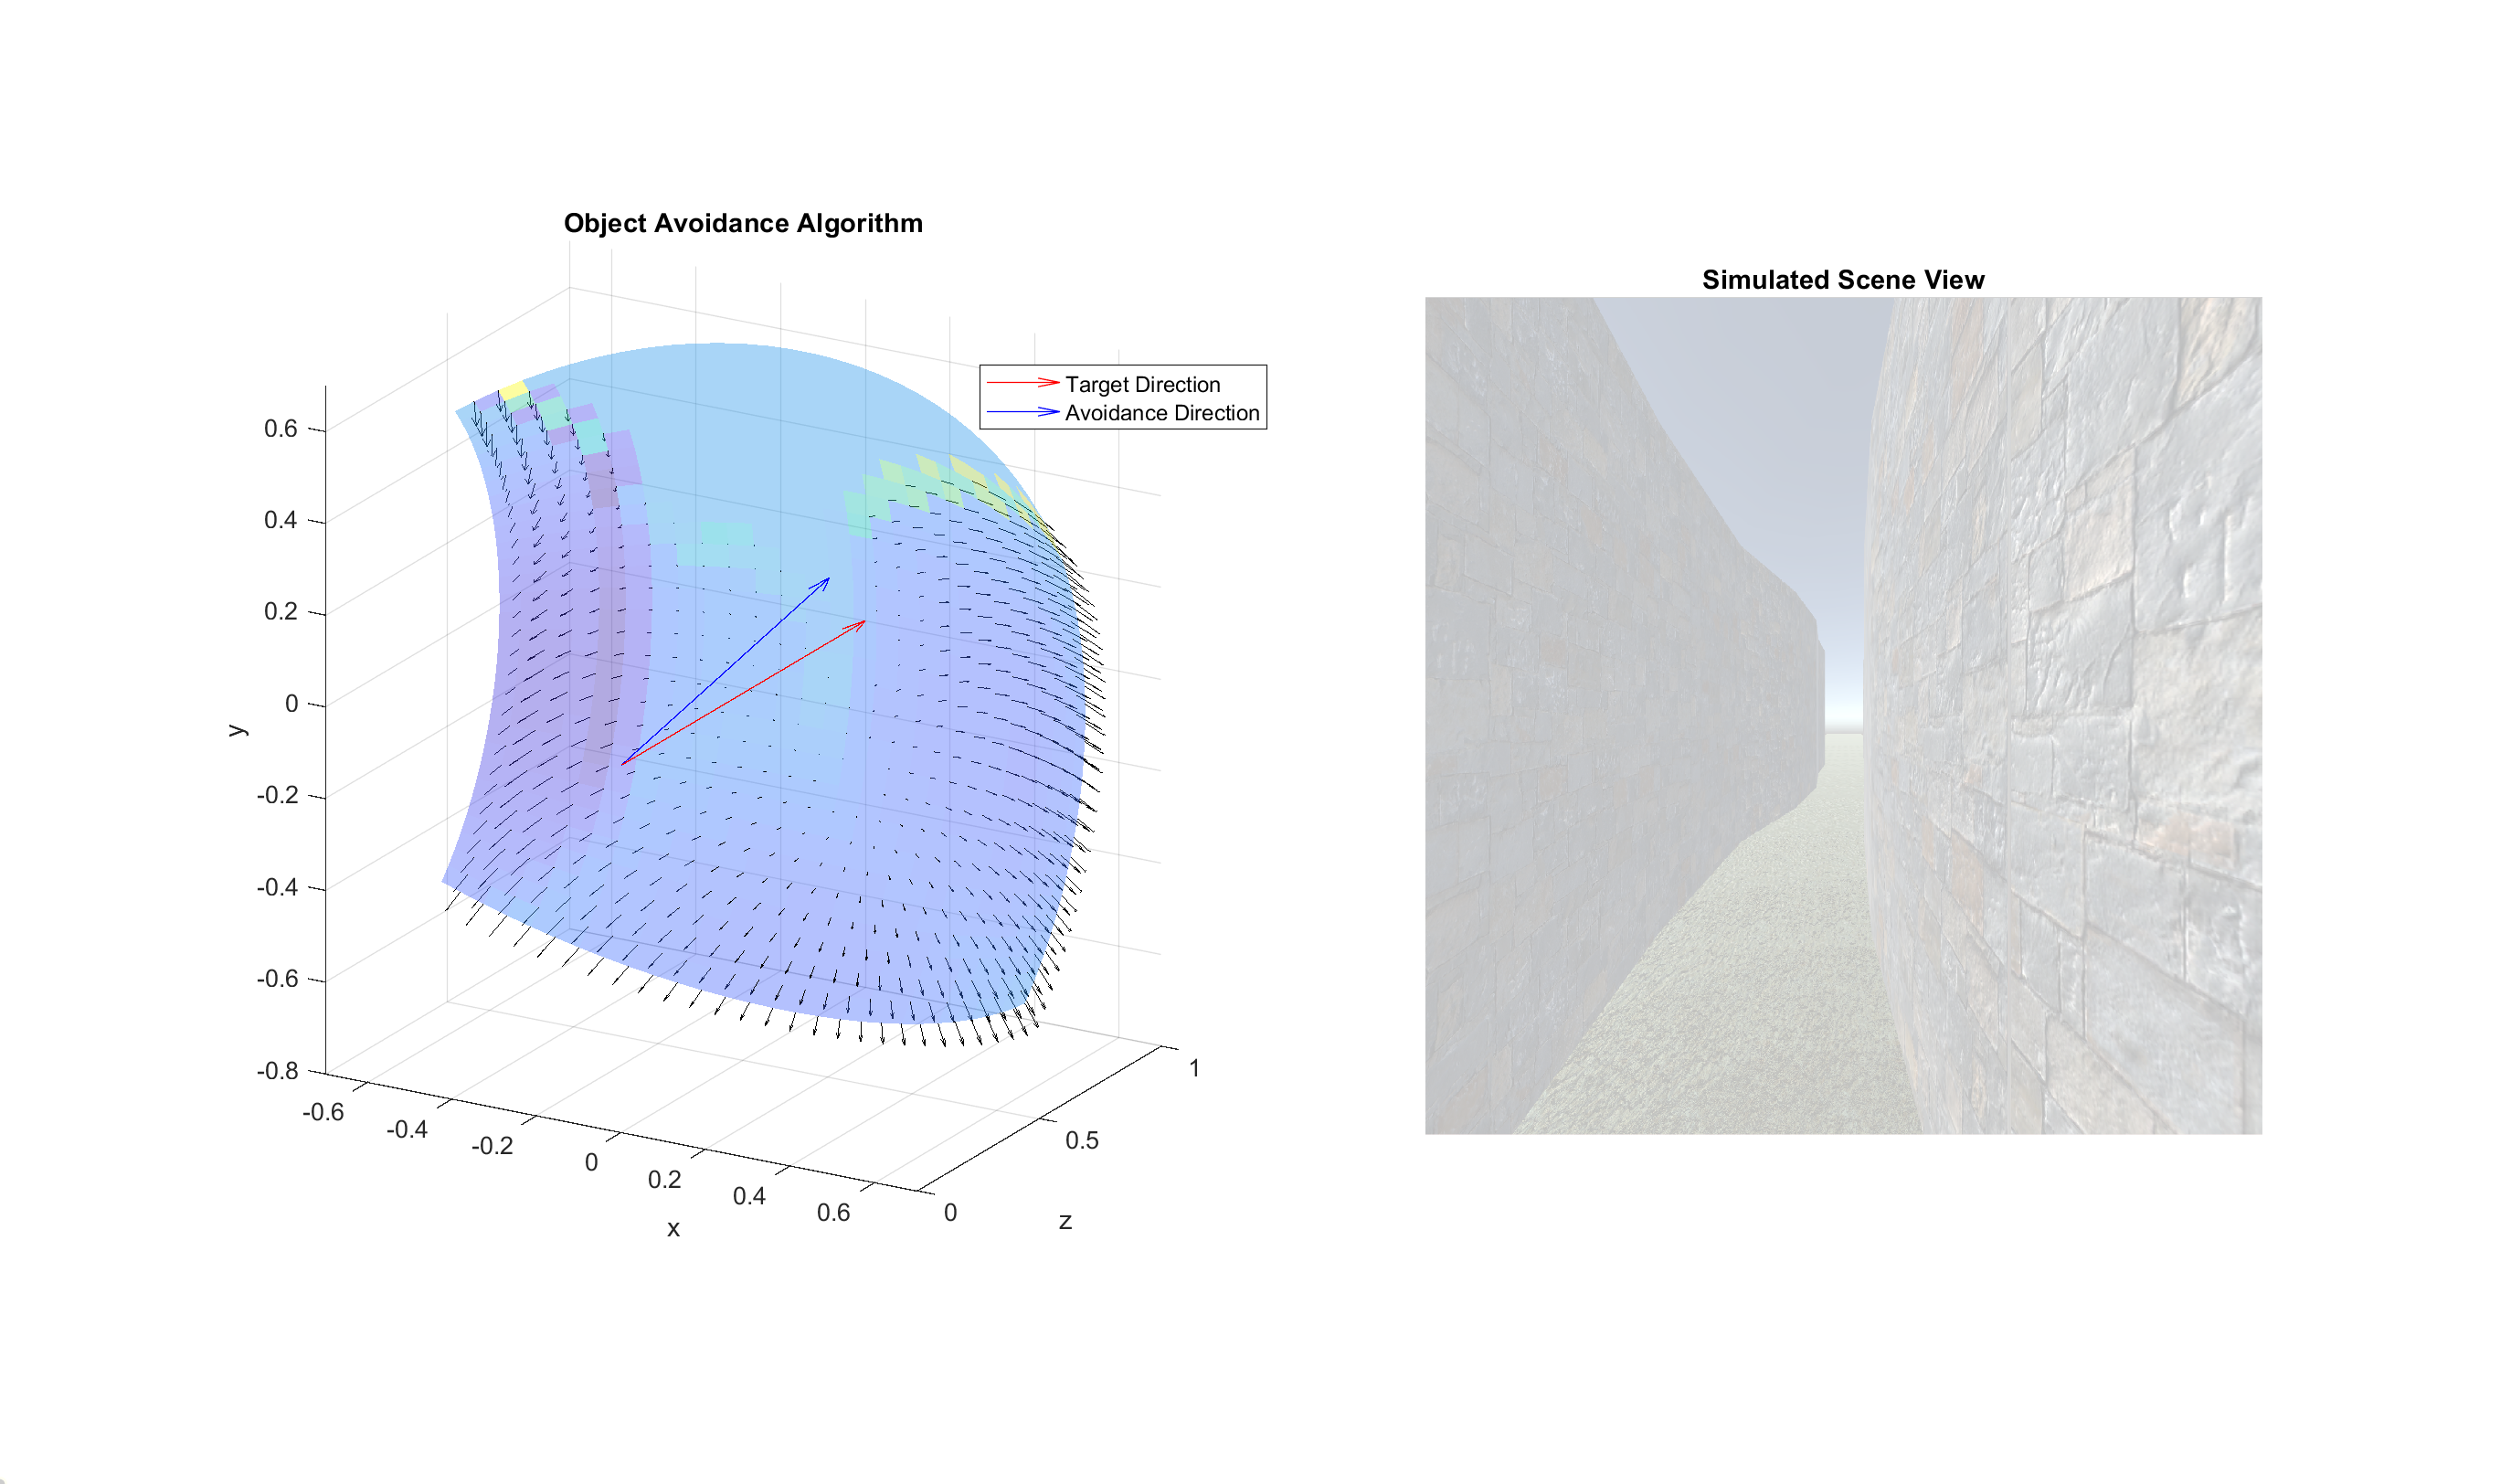
\includegraphics[width=.8\linewidth]{Figures/Matlab/Avoidance_Algorithm}
        \caption{Caption}
        \label{fig:Avoidance_Algorithm}
    \end{center}
\end{figure}

%%%%%%%%%%%%%%%%%%%%%%%%%%%%%%%
\newpage
\section{Discussion}
Environment navigation is an extremely broard topic, and this project contributes a small amout towards the obstacl avoidance 
%%%%%%%%%%%%%%%%%%%%%%%%%%%%%%%
\newpage
\section{Conclusion}\label{sec:Conclusion}
The goal of this project was to investigate the plausability of using optical flow cues as a method for avoiding obstacles in a scene. Results of the simulations show that the a cost function based on divergence of an optical flow field generates a suitable control policy, stearing the UAV in a direction away from obstacles such as walls and buildings. 

%%%%%%%%%%%%%%%%%%%%%%%%%%%%%%%
\newpage
\section{Recomendations}
For the results of this project to be implemented on a robotic platform, an optical flow algoithm would need to be run in real time. for this, an image flow algorithm that can be implemented on a descrete graphic card should be implemented such as that ceated by \cite{adarve2016filter}.


%%%%%%%%%%%%%%%%%%%%%%%%%%%%%%%
\newpage
\bibliographystyle{harvard}
\bibliography{main} % This is the .bib file where the bibliography database is stored

%%%%%%%%%%%%%%%%%%%%%%%%%%%%%%%
\appendix
\newpage
\section{Journal}\label{app:Journal}
\newpage
\section{Calibration Tool}\label{app:calibrationTool}
\begin{figure}[ht]
    \begin{center}
        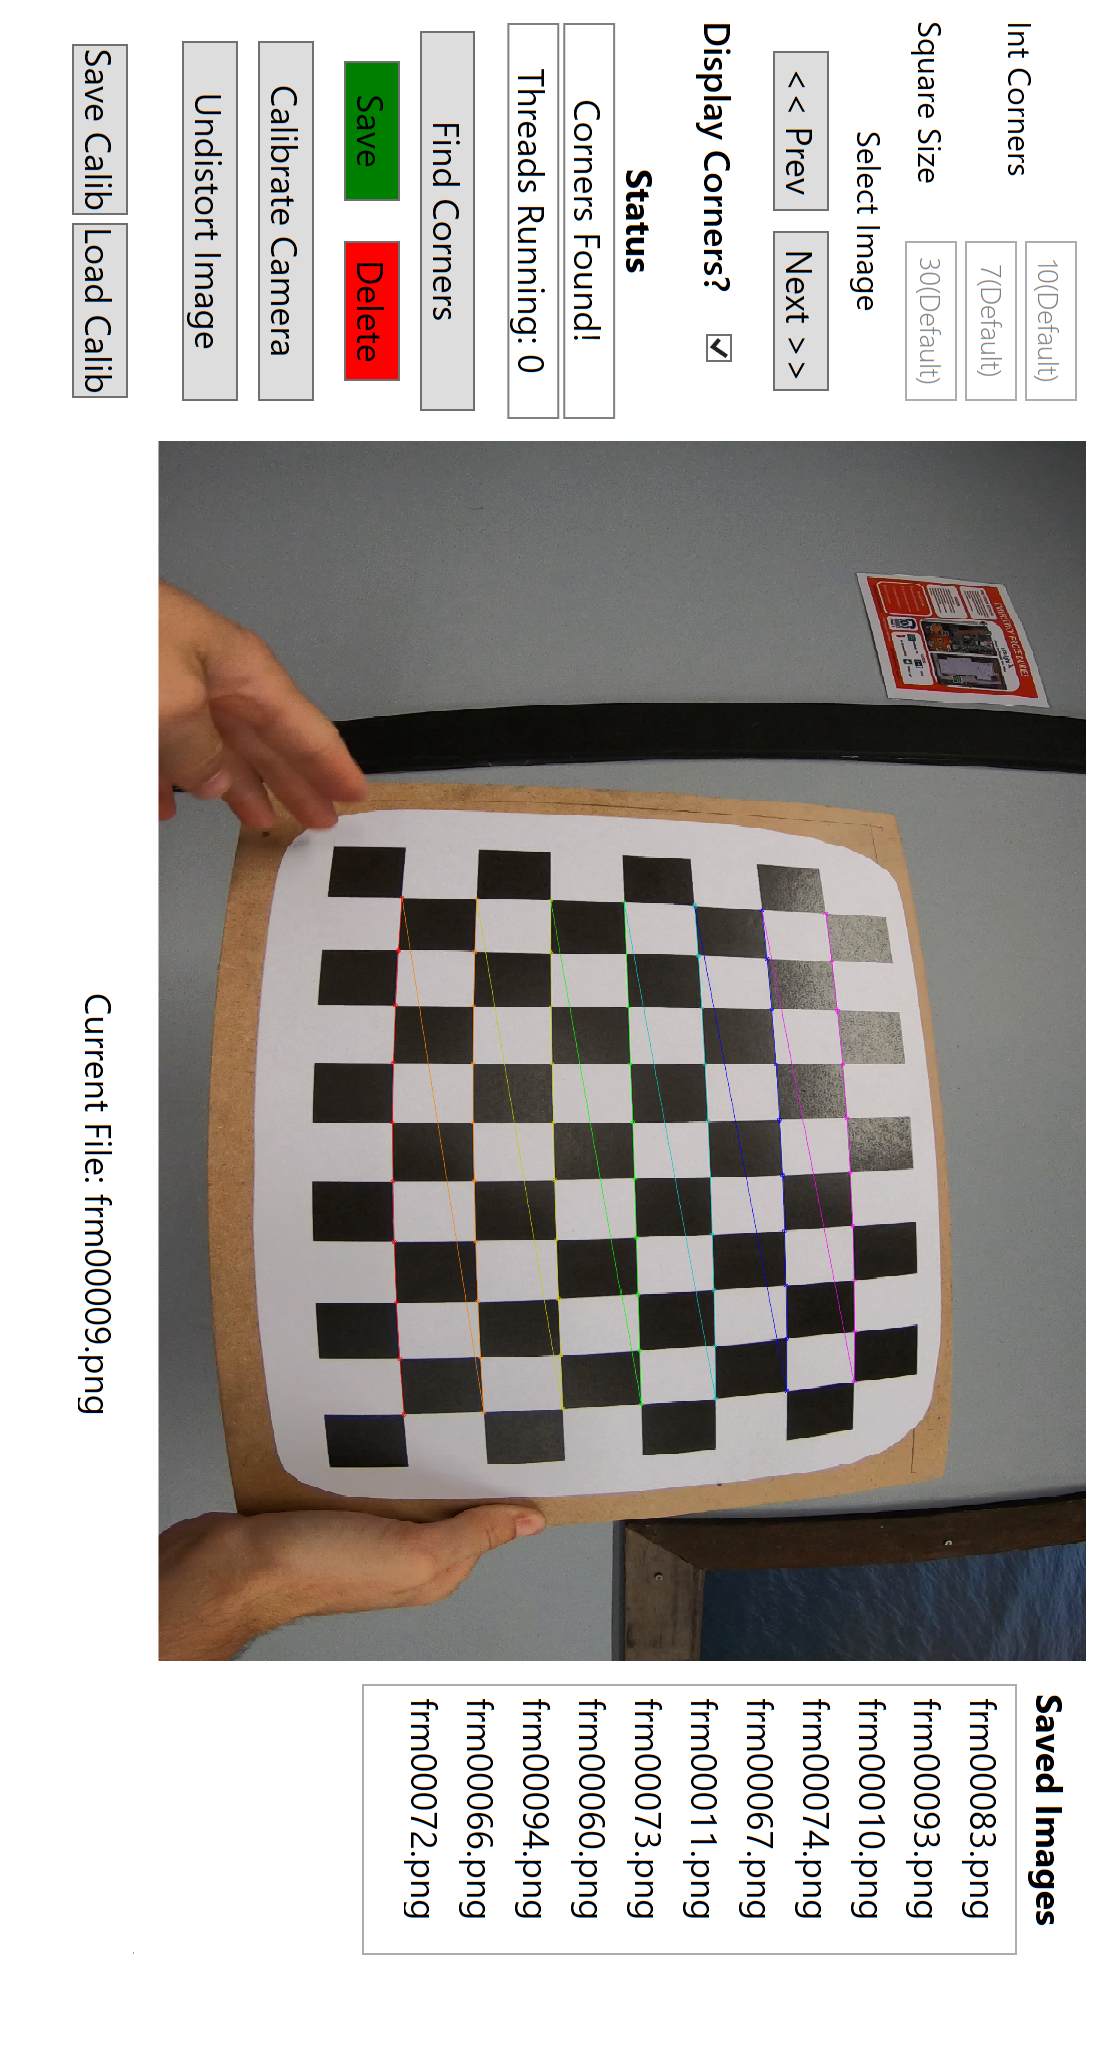
\includegraphics[width=.5\linewidth]{Figures/Calibration_Tool}
        \caption{Write something here}
        \label{fig:Calibration_Tool}
    \end{center}
\end{figure}
\newpage
\section{Calibration Board}\label{app:calibrationBoard}
\begin{figure}[ht]
    \begin{center}
        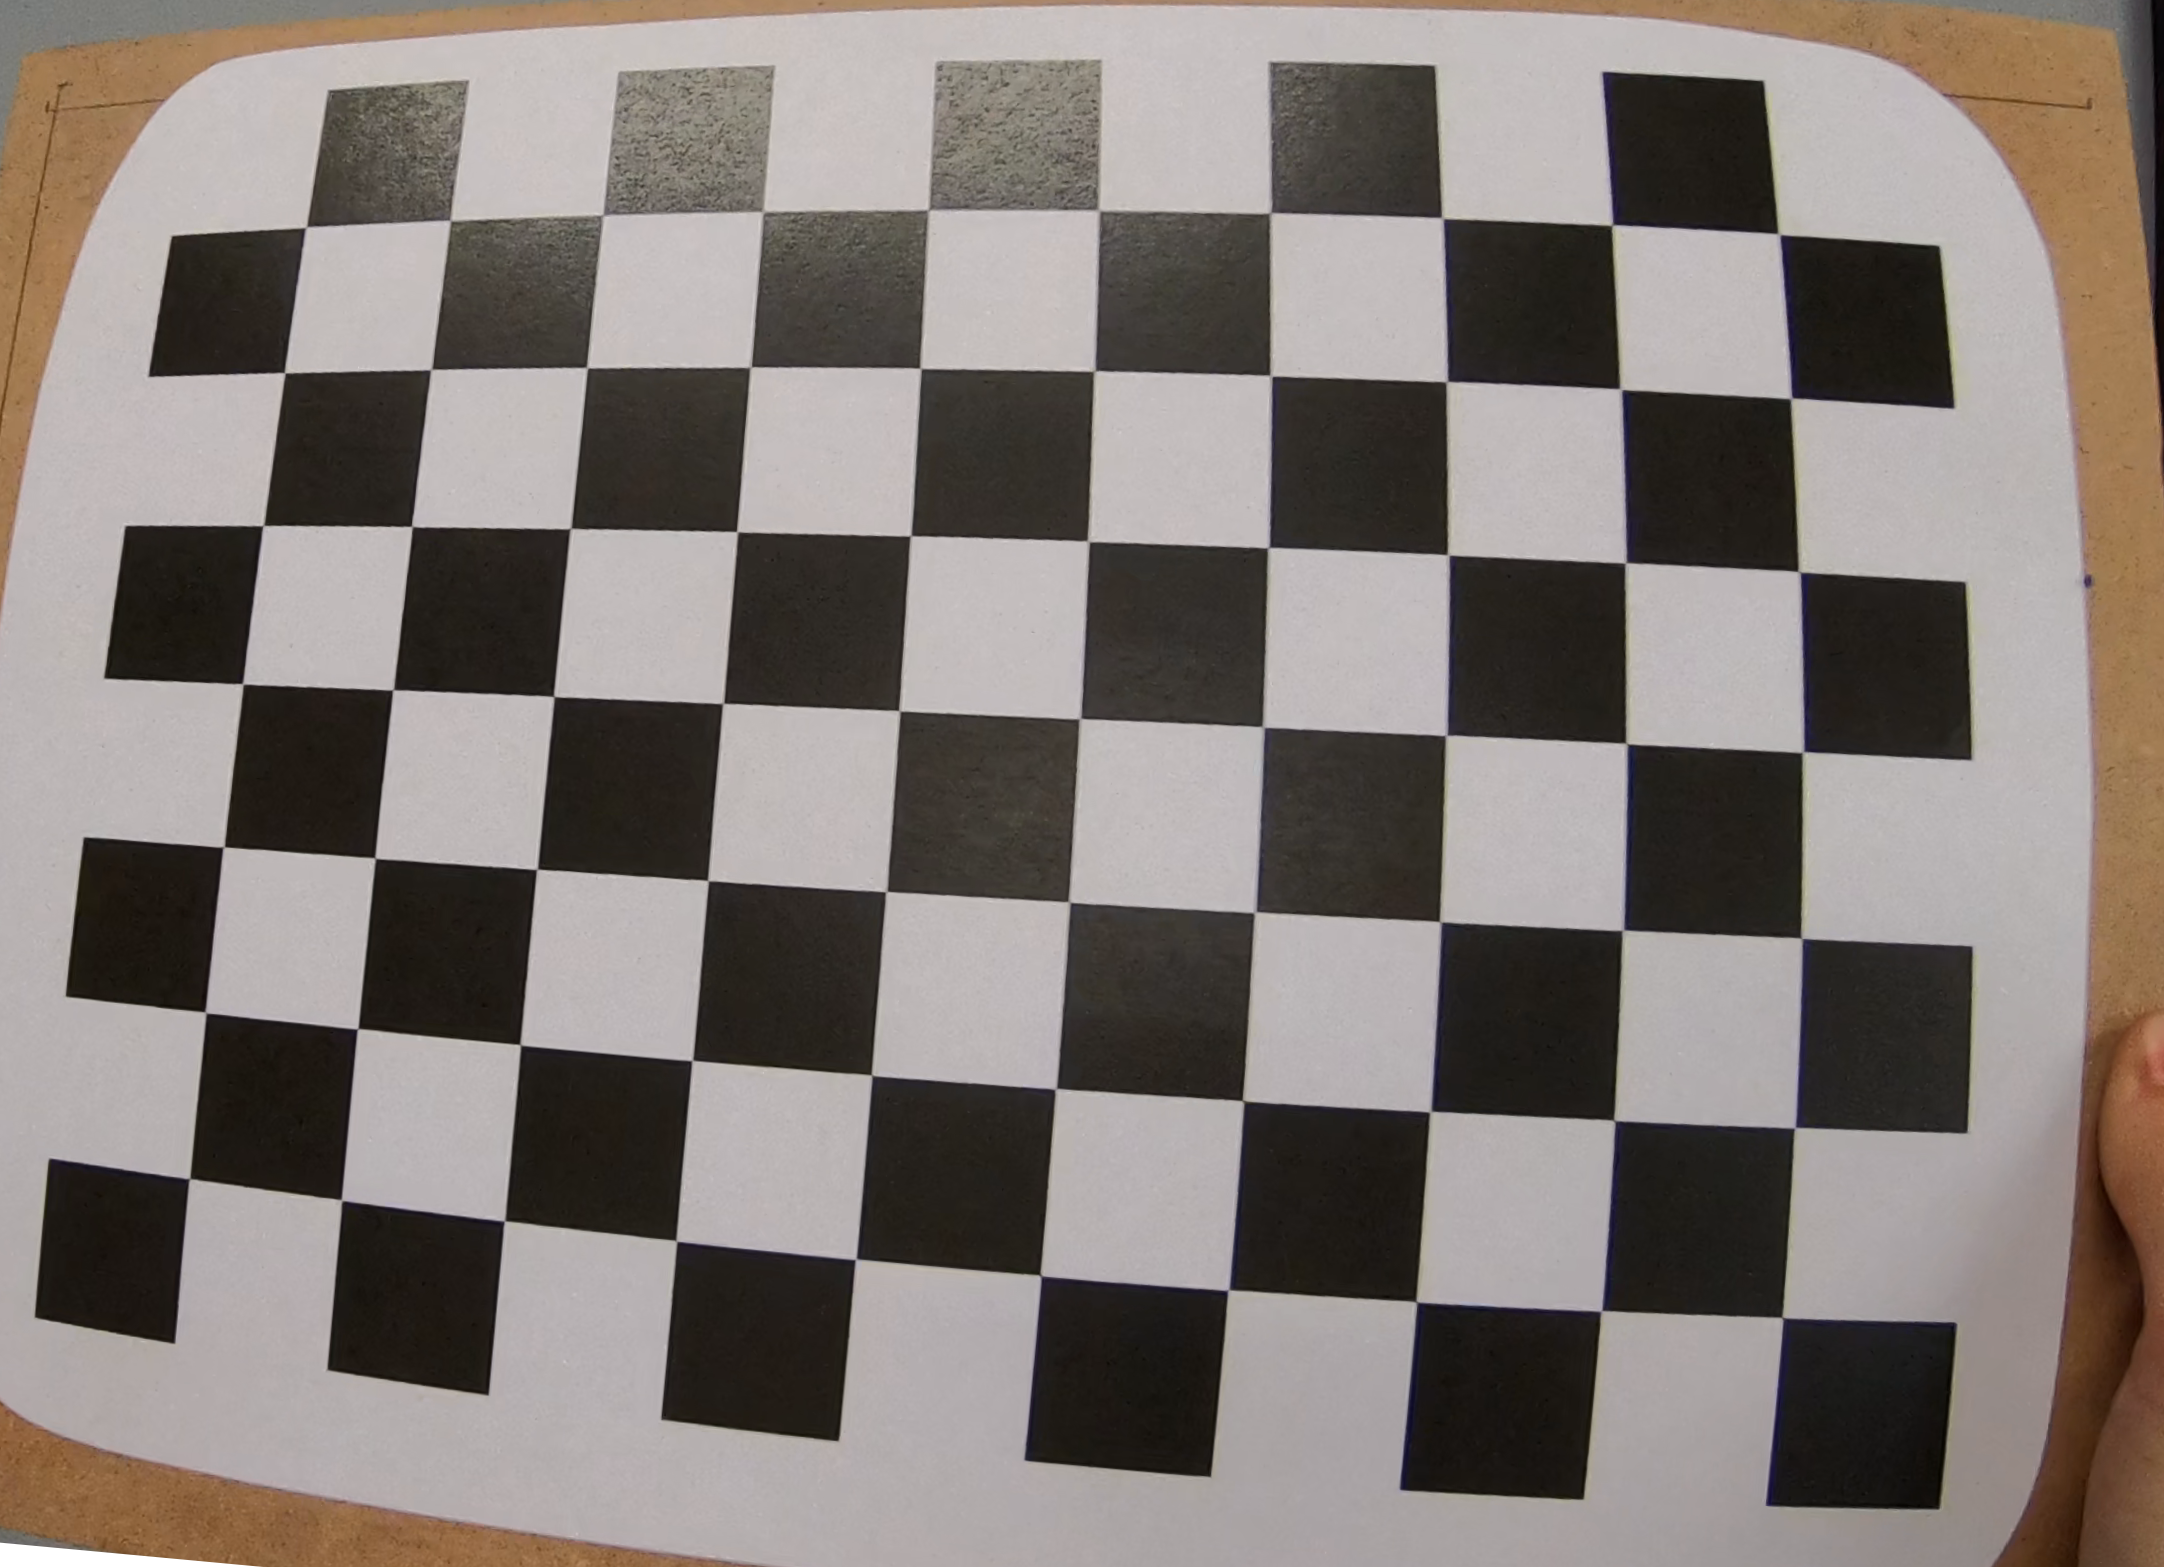
\includegraphics[width=.6\linewidth]{Figures/calibrationBoard}%TODO: change this to a pictiure of unity
        \caption{Calibration pattern mounted to a rigid MDF board, creating a rigid pattern the calibration process can reference}
        \label{fig:UnityEnvironment}
    \end{center}
\end{figure}
\newpage
\section{Unity environment}\label{app:unityEnvironment}
\begin{figure}[ht]
    \begin{center}
        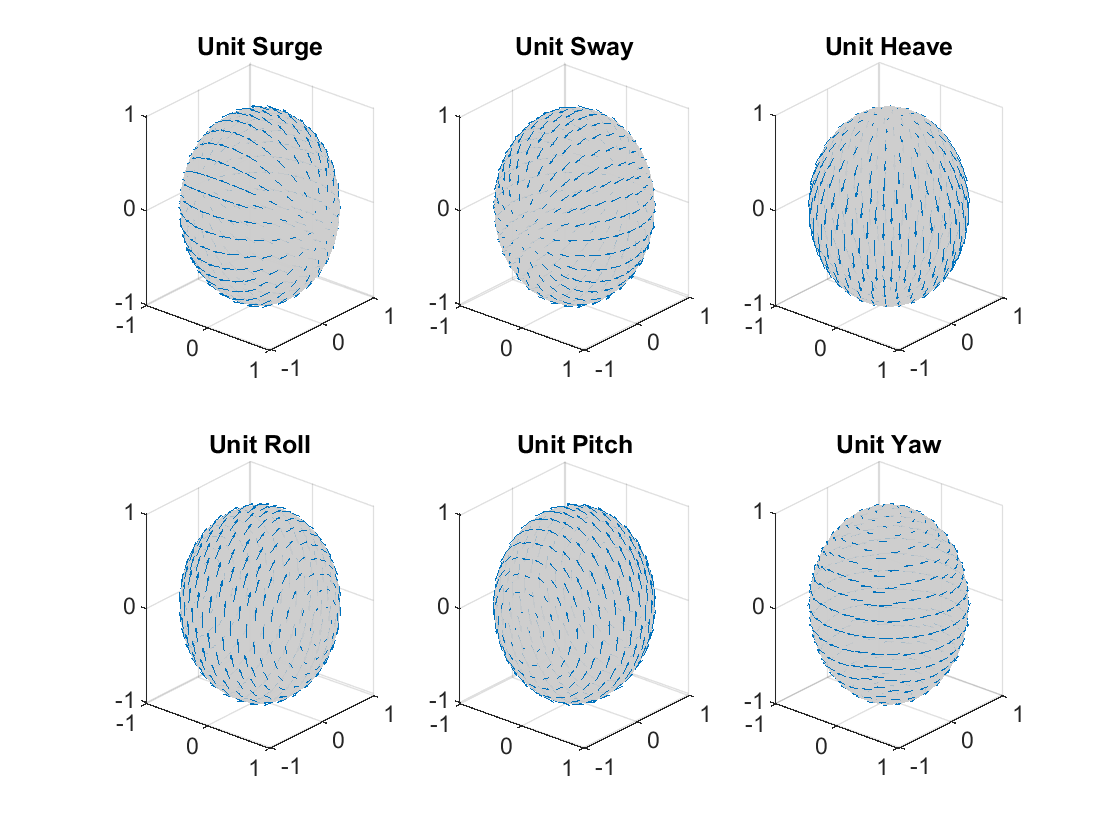
\includegraphics[width=.6\linewidth]{Figures/Unit_Movement}%TODO: change this to a pictiure of unity
        \caption{Write something here}
        \label{fig:UnityEnvironment}
    \end{center}
\end{figure}

\end{document}